\chapter{CONCLUSION AND ANALYSIS}
\section{Conclusion}
LabXplorerX is an innovative virtual laboratory platform tailored for enhancing science education through interactive simulations and experiments. It aims to revolutionize how students and educators engage with scientific concepts by offering a diverse range of features. LabXplorerX facilitates seamless exploration, collaboration, and learning aweb various scientific disciplines. This platform empowers users to conduct experiments, share insights, and leverage sophisticated algorithms to deepen their understanding. Additionally, LabXplorerX integrates advanced reporting capabilities and decision-making tools, enriching the educational experience beyond traditional classroom settings.
\\section{Lesson Learned / Outcome}

The LabXplorerX project has made substantial progress in developing an interactive platform that fosters educational engagement. Throughout this journey, several key lessons have been learned:

\begin{itemize}[leftmargin=1cm]
    \item \textbf{Creating Engaging Simulations:} The development of 5 interactive simulations (Gravity Simulator, Ohm's Law Simulator, Atom Simulator, Solar System Simulator, and JavaScript Editor) has shown the value of hands-on learning tools. These simulations have proven effective in transforming abstract concepts into practical, experiential learning opportunities, greatly enhancing student understanding.
    
    \item \textbf{Content Design through Learning Capsules:} The creation of structured learning capsules highlighted the importance of organizing content into manageable, interactive modules. These capsules, while lacking visual aids, demonstrated that well-structured, interactive content is sufficient to foster student engagement and deeper understanding across various educational subjects.
    
    \item \textbf{Secure Authentication Systems:} Implementing a robust authentication system revealed the critical role of secure access management. Secure login, registration, and account management features are not only essential for protecting user data but also for building trust between students, teachers, and administrators. 
    
    \item \textbf{Centralized Admin Panel:} The creation of a comprehensive admin panel underscored the need for efficient management tools. By allowing administrators to manage capsules, quizes and simulations, the panel ensures streamlined operations and platform sustainability.
    
    \item \textbf{Quizzes for Self-assessment:} Integrating quizzes into the learning modules provided valuable insight into the importance of continuous self-assessment. These quizzes enabled students to evaluate their grasp of the material, offering immediate feedback and enhancing the learning process.
    
    \item \textbf{User-centric Interface Design:} The development of various user interface screens (Home Screen, Login Screen, Register Screen, Simulations Screen, etc.) highlighted the significance of intuitive design. A user-friendly interface is key to an accessible and engaging learning experience, ensuring both students and teachers can easily navigate the platform.
\end{itemize}

All planned features have been successfully implemented, providing a secure, interactive, and engaging platform for learning. These lessons will guide future improvements, helping to maintain LabXplorerX as a leading educational tool.

\newpage
\subsection{Screenshots of Outcomes}
% Home Screen
\textbf{Home Screen:} Below is the screenshot of the Home Screen, which is the main interface of the application.
\begin{figure}[H]
    \centering
    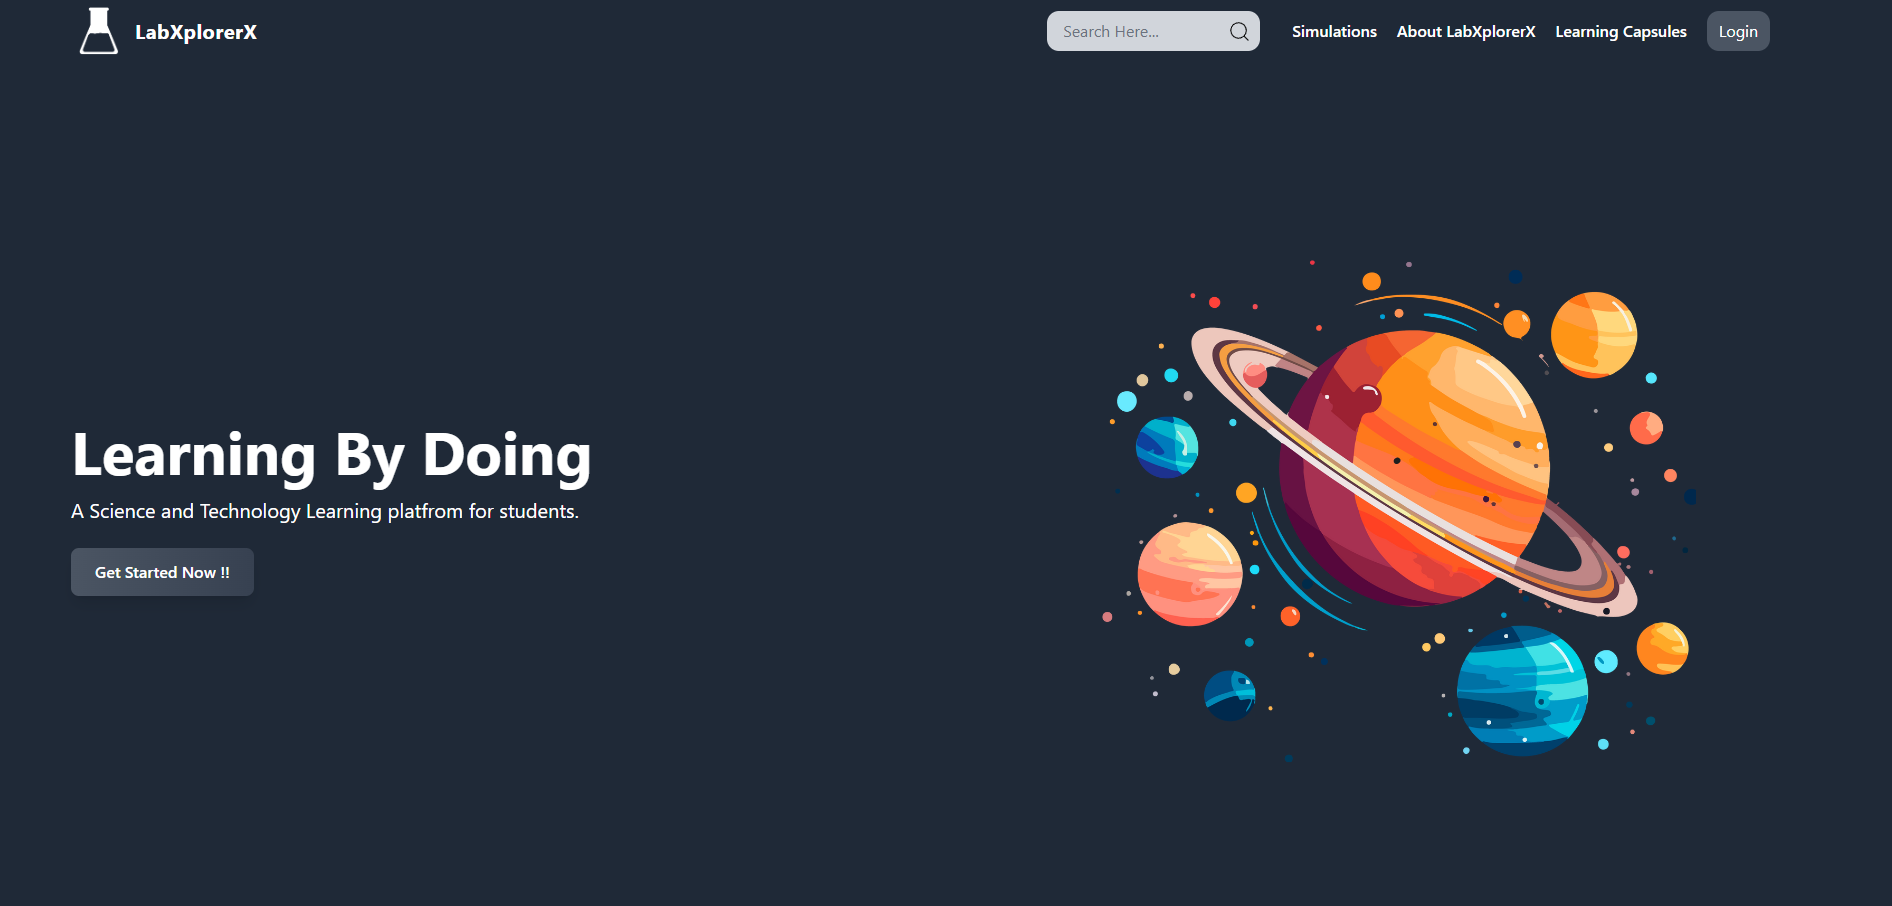
\includegraphics[width = 14cm]{Diagrams/output/home.png}
    \caption{Home Screen}
\end{figure}

% Login Screen
\textbf{Login Screen:} Below is the screenshot of the Login Screen, where users enter their credentials to access their accounts.
\begin{figure}[H]
    \centering
    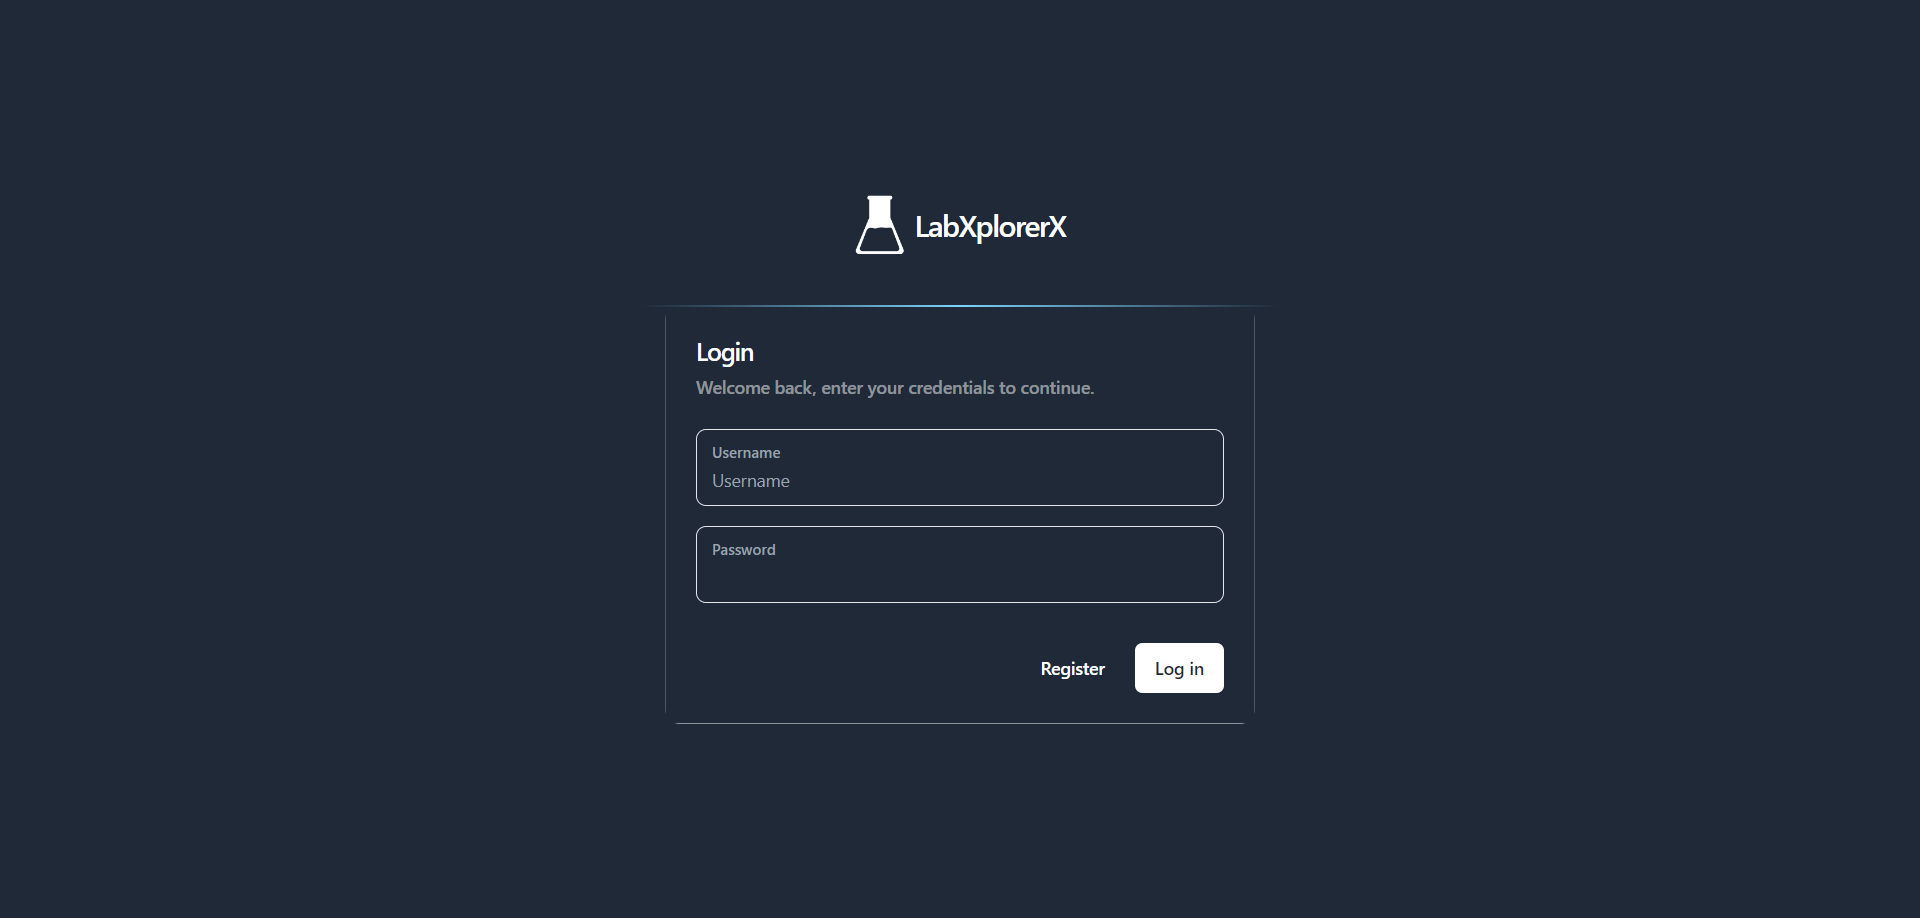
\includegraphics[width = 15cm]{Diagrams/output/login.png}
    \caption{Login}
\end{figure}
\newpage
% Register Screen
\textbf{Register Screen:} Below is the screenshot of the Register Screen, where new users can create an account.
\begin{figure}[H]
    \centering
    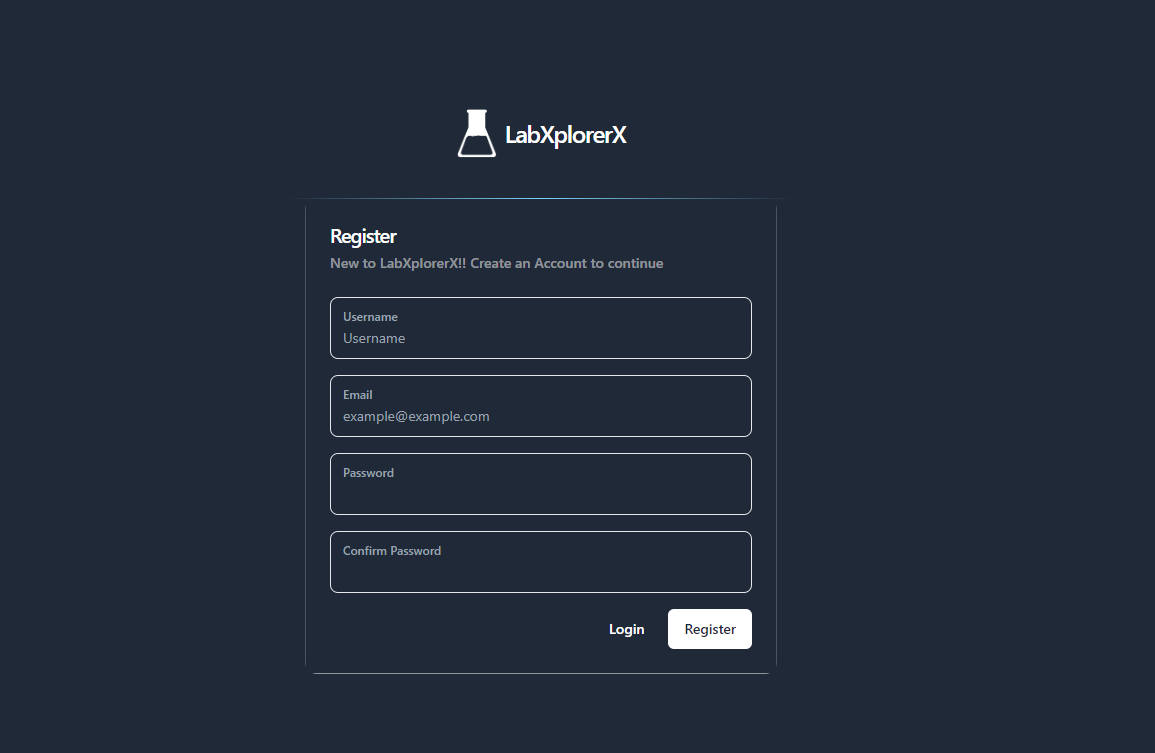
\includegraphics[width = 16cm]{Diagrams/output/register.png}
    \caption{Register}
\end{figure}

% About Page
\textbf{About Page:} Below is the screenshot of the About Page, which provides information about the application.
\begin{figure}[H]
    \centering
    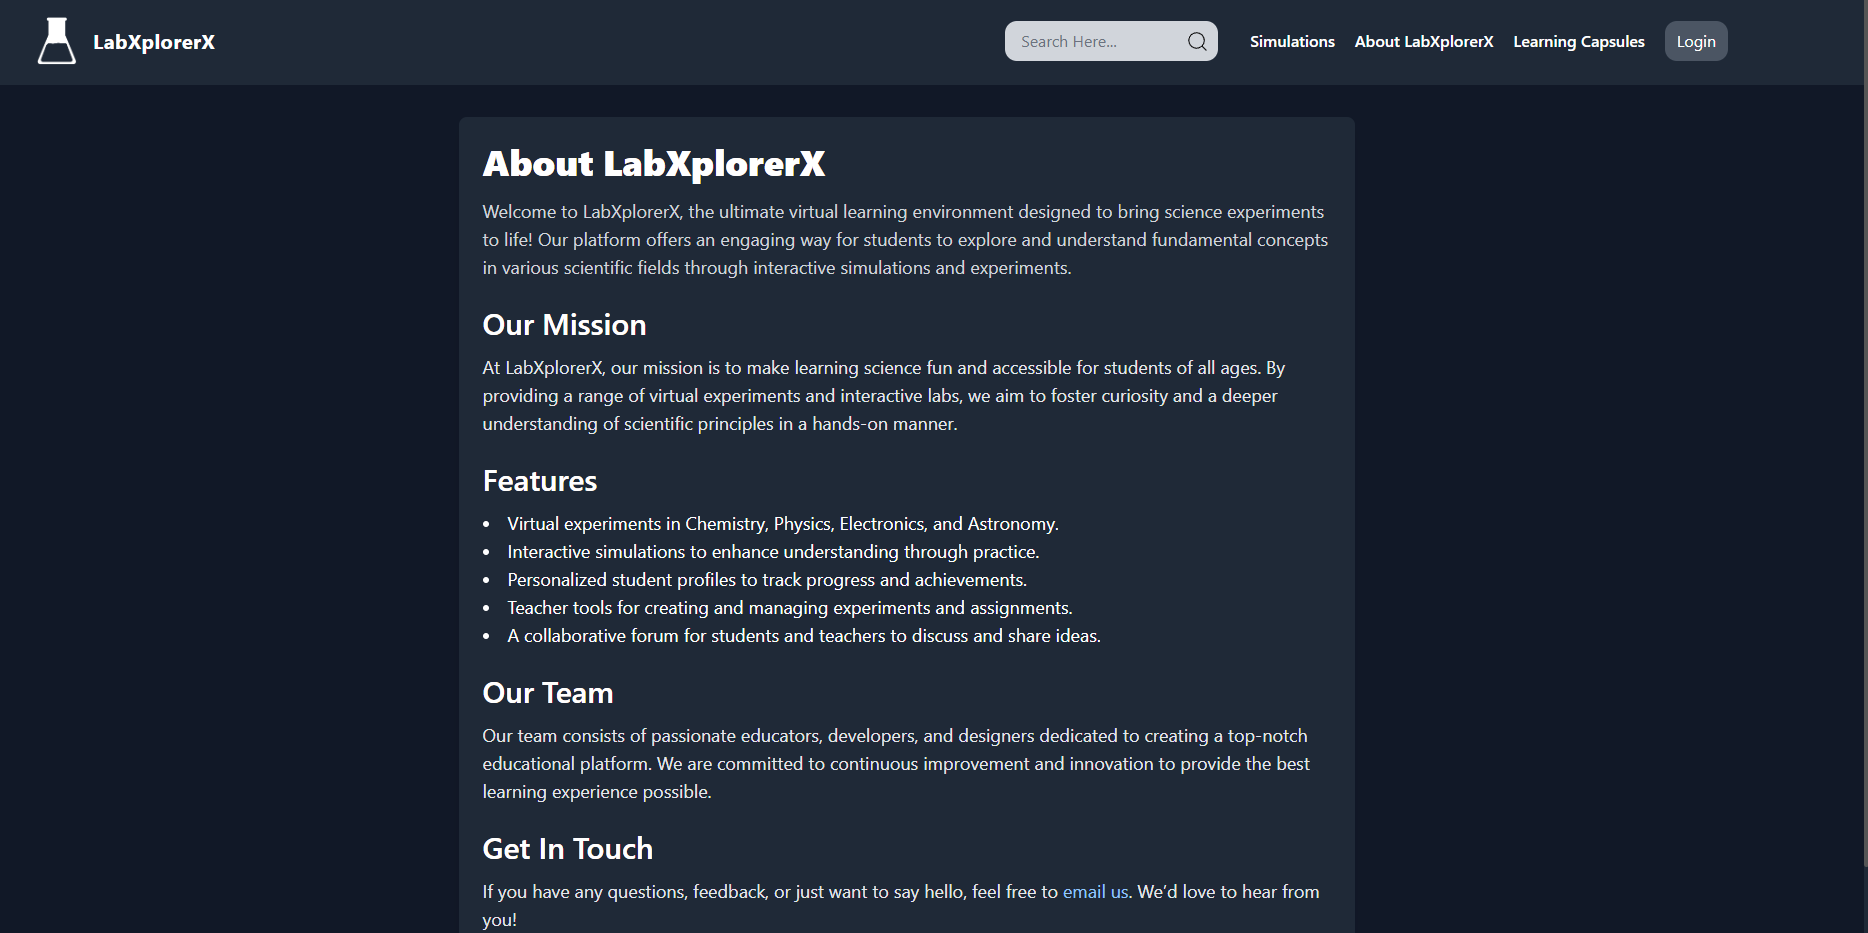
\includegraphics[width = 16cm]{Diagrams/output/about.png}
    \caption{About Page}
\end{figure}
\newpage

% Learning Areas Screen
\textbf{Learning Areas Screen:} Below is the screenshot of the Learning Areas Screen, showing the various educational categories available.
\begin{figure}[H]
    \centering
    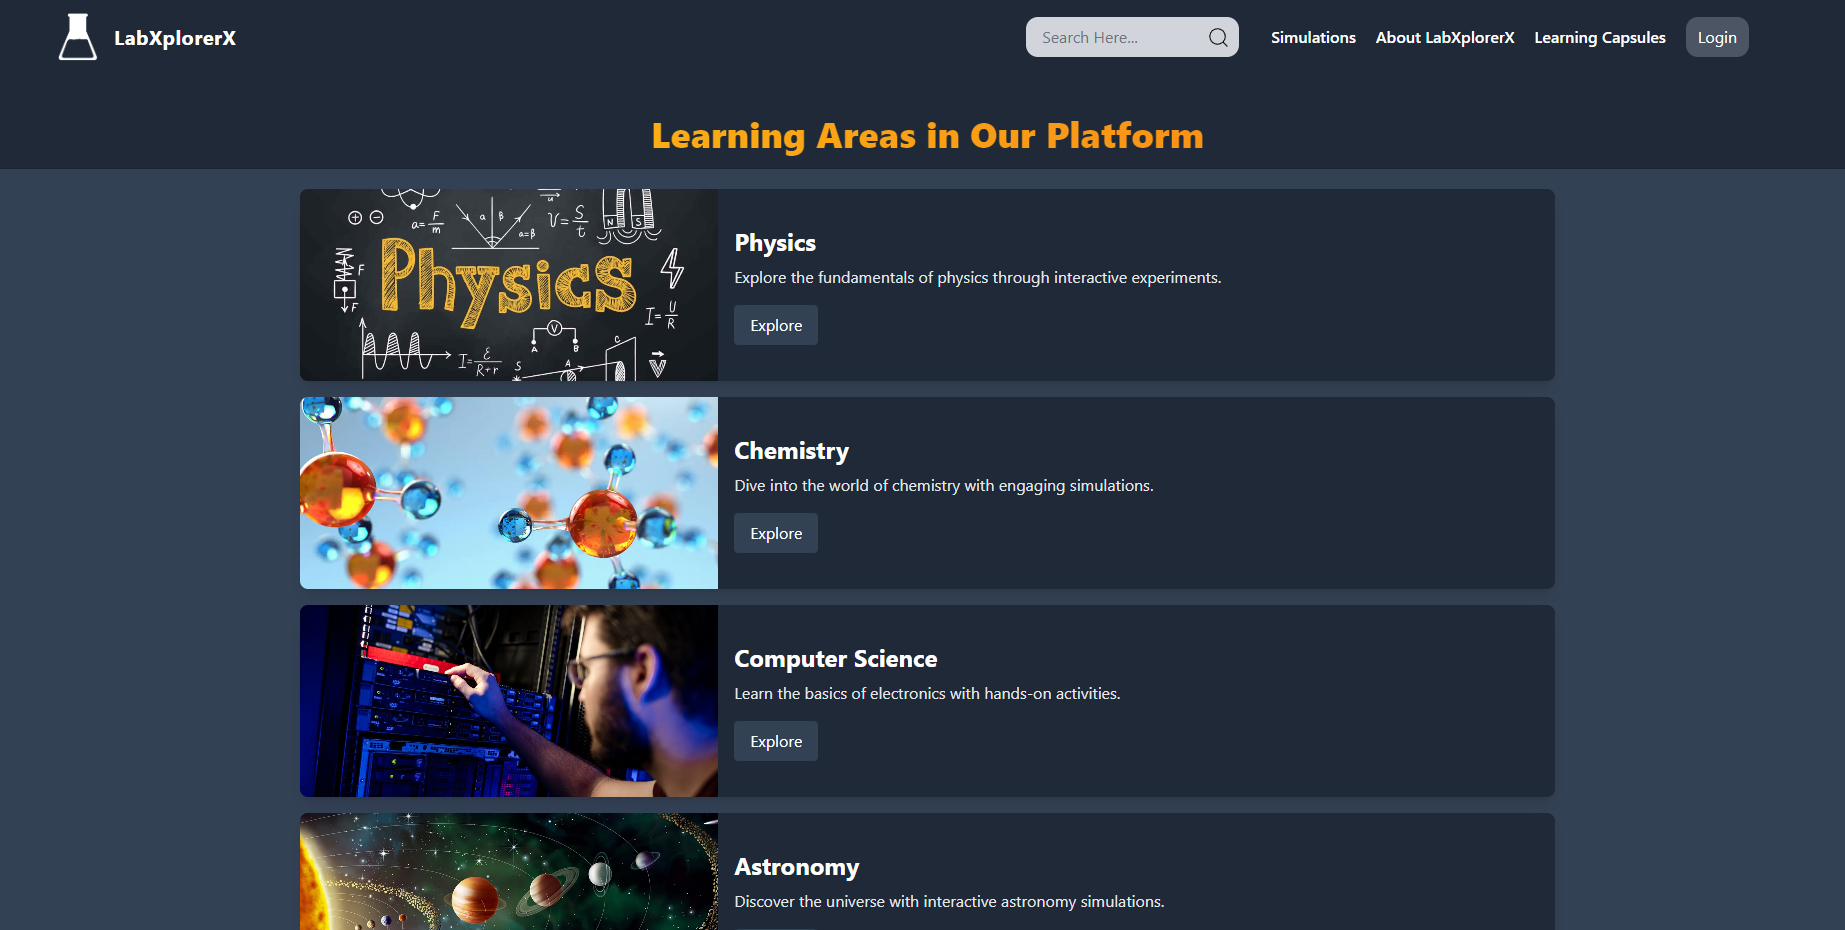
\includegraphics[width = 15cm]{Diagrams/output/learningareas.png}
    \caption{Learning Areas}
\end{figure}

% Simulations Screen
\textbf{Simulations Screen:} Below is the screenshot of the Simulations Screen, where users can access different simulations.
\begin{figure}[H]
    \centering
    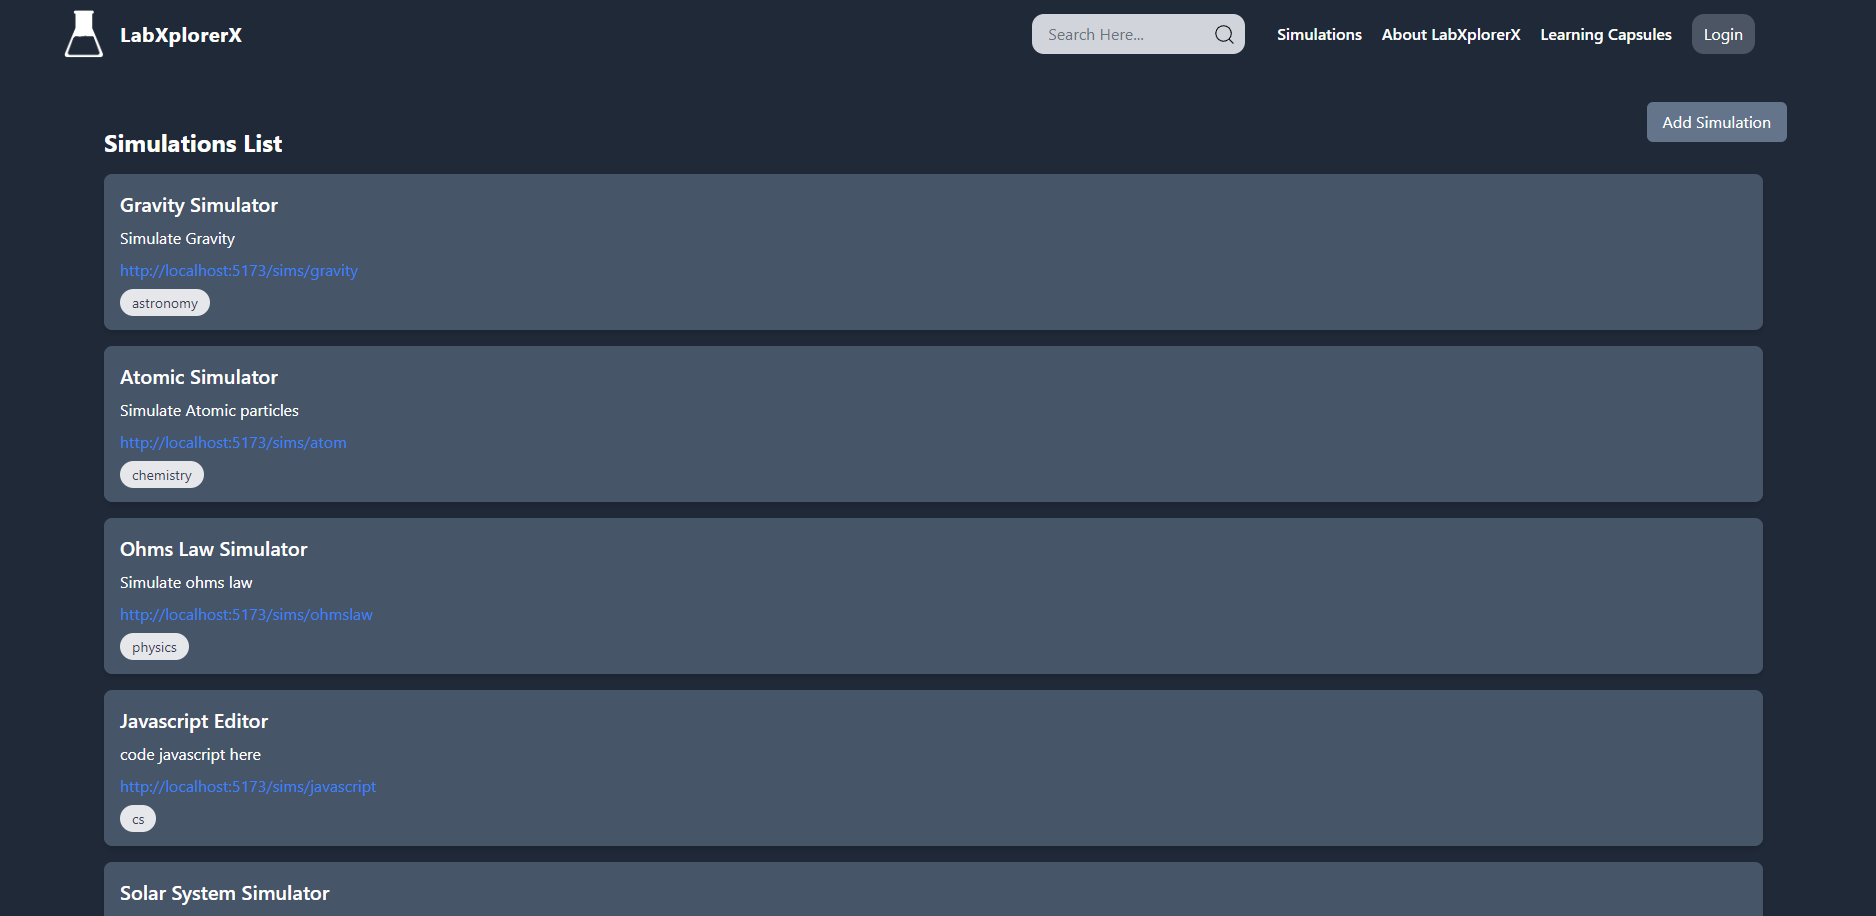
\includegraphics[width = 15cm]{Diagrams/output/simulations.png}
    \caption{Simulations}
\end{figure}

% Capsules Screen
\textbf{Capsules Screen:} Below is the screenshot of the Capsules Screen, which displays the available capsules in the application.
\begin{figure}[H]
    \centering
    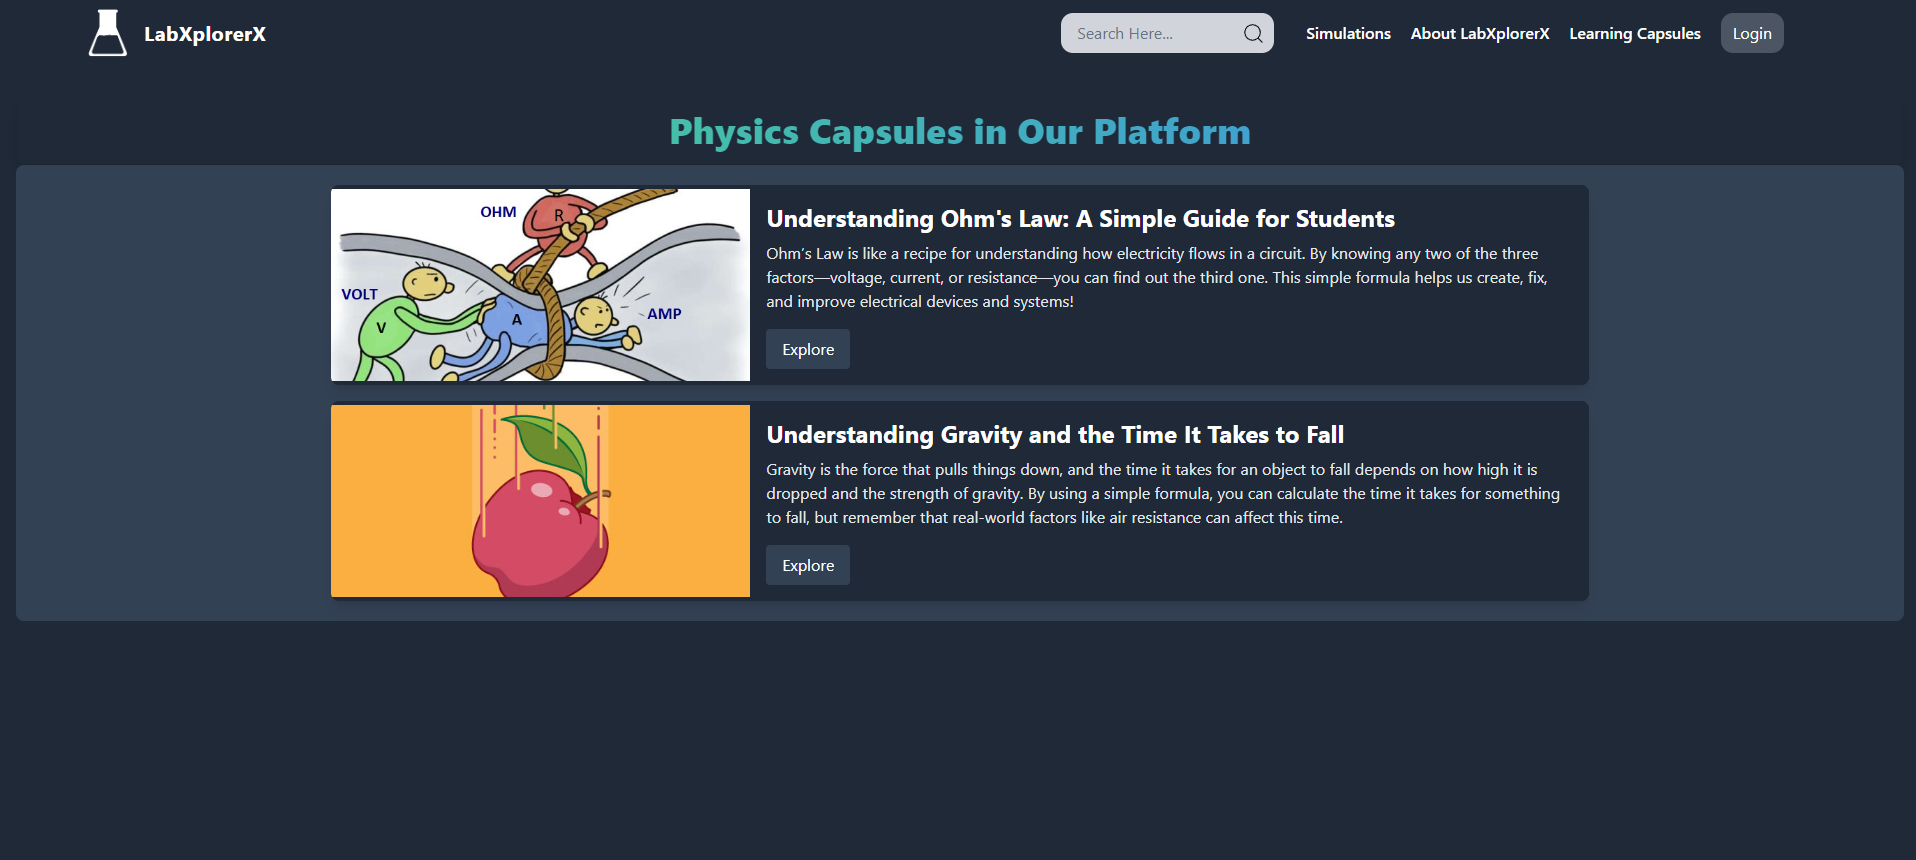
\includegraphics[width = 16cm]{Diagrams/output/capsules.png}
    \caption{Capsules}
\end{figure}

% Quizzes Screen
\textbf{Quizzes Screen:} Below is the screenshot of the Quizzes Screen, where users can participate in various quizzes.
\begin{figure}[H]
    \centering
    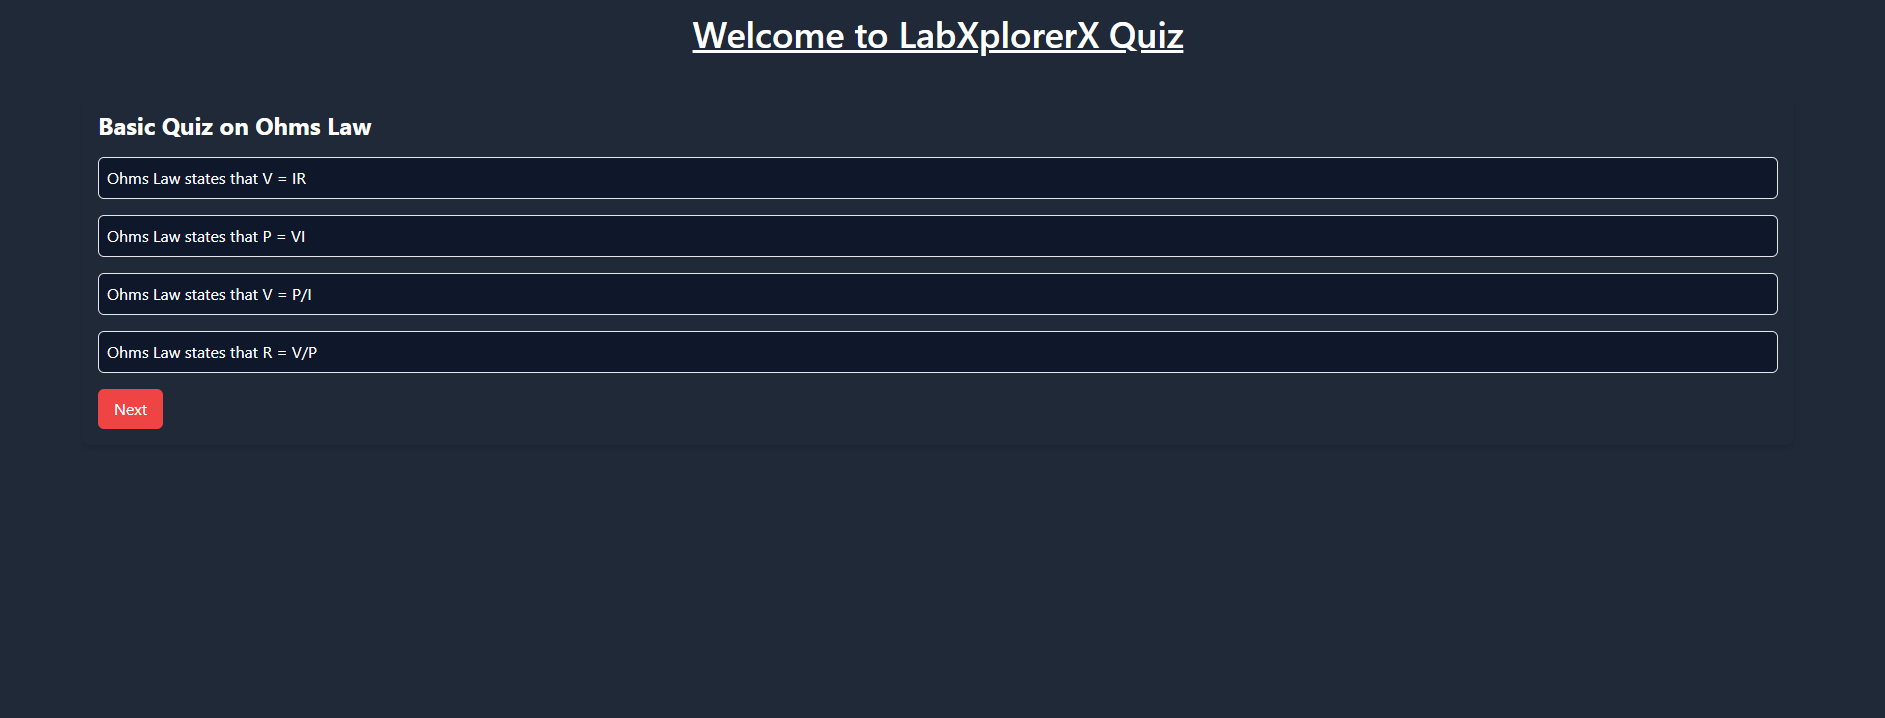
\includegraphics[width = 16cm]{Diagrams/output/quiz.png}
    \caption{Quizzes}
\end{figure}
\newpage

% Admin Panel
\textbf{Admin Panel:} Below is the screenshot of the Admin Panel, used by administrators to manage the application.
\begin{figure}[H]
    \centering
    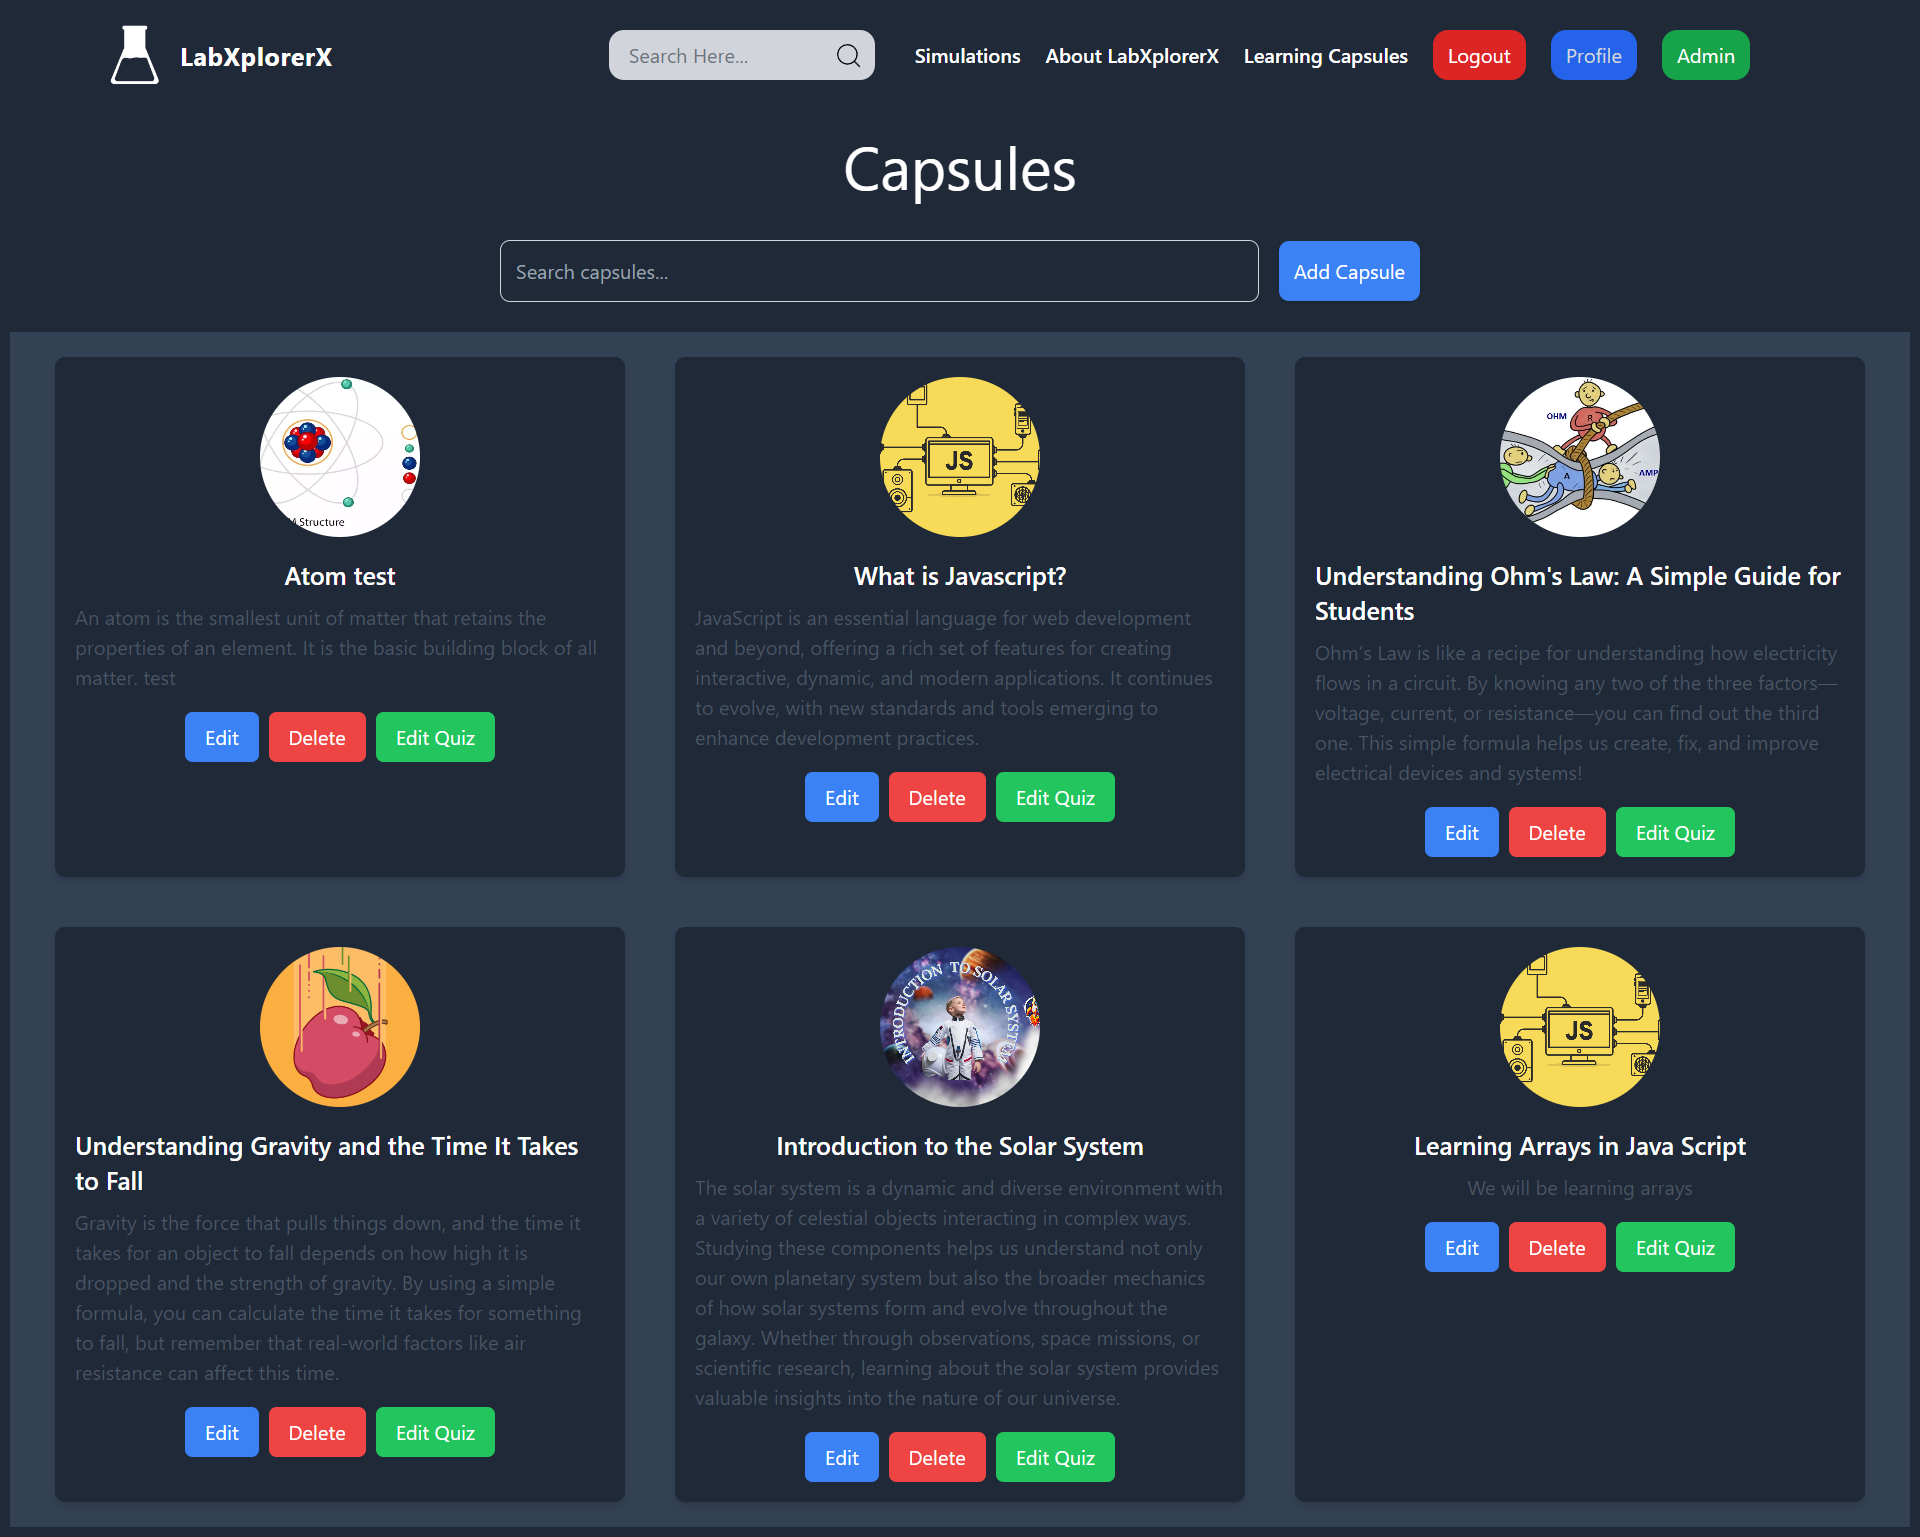
\includegraphics[width = 16cm]{Diagrams/output/admin.png}
    \caption{Admin Panel}
\end{figure}
\newpage

% Add Simulations Screen
\textbf{Add Simulations Screen:} Below is the screenshot of the Add Simulations Screen, where administrators can add new simulations.
\begin{figure}[H]
    \centering
    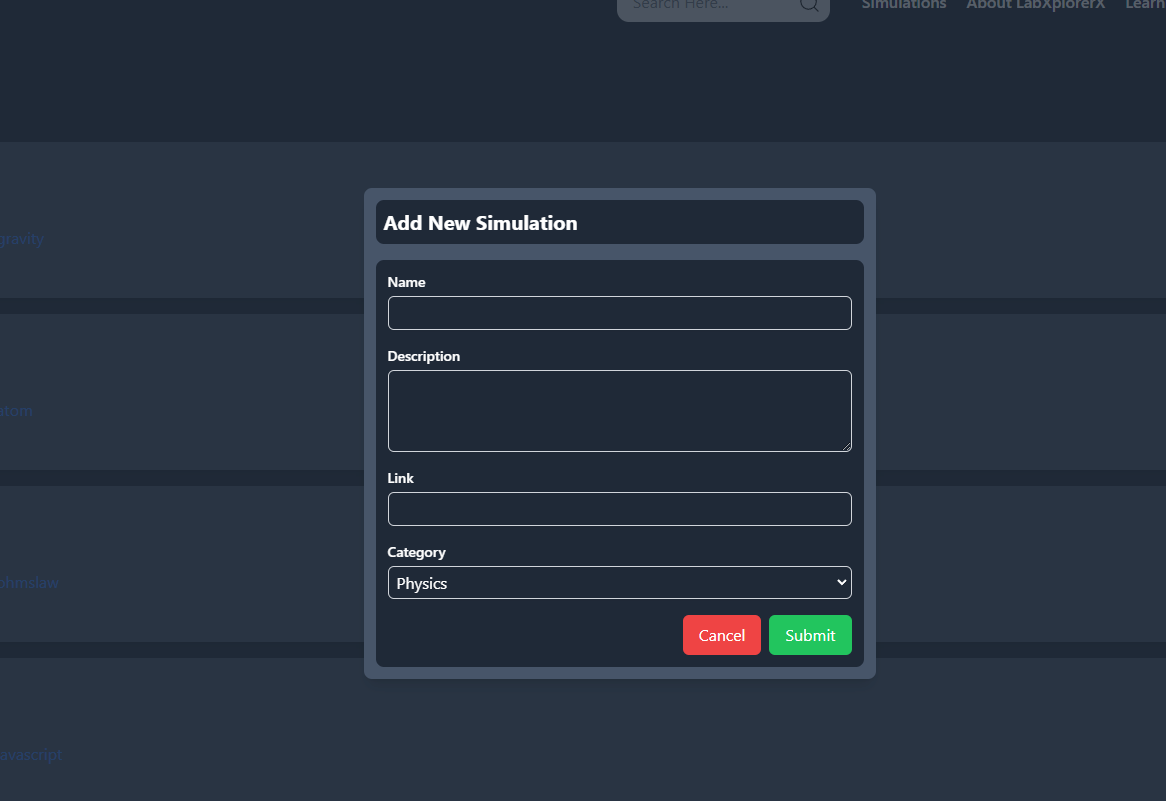
\includegraphics[width = 15cm]{Diagrams/output/addsimulations.png}
    \caption{Add Simulations}
\end{figure}

% Profile Screen
\textbf{Profile Screen:} Below is the screenshot of the Profile Screen, where users can view and edit their profile information.
\begin{figure}[H]
    \centering
    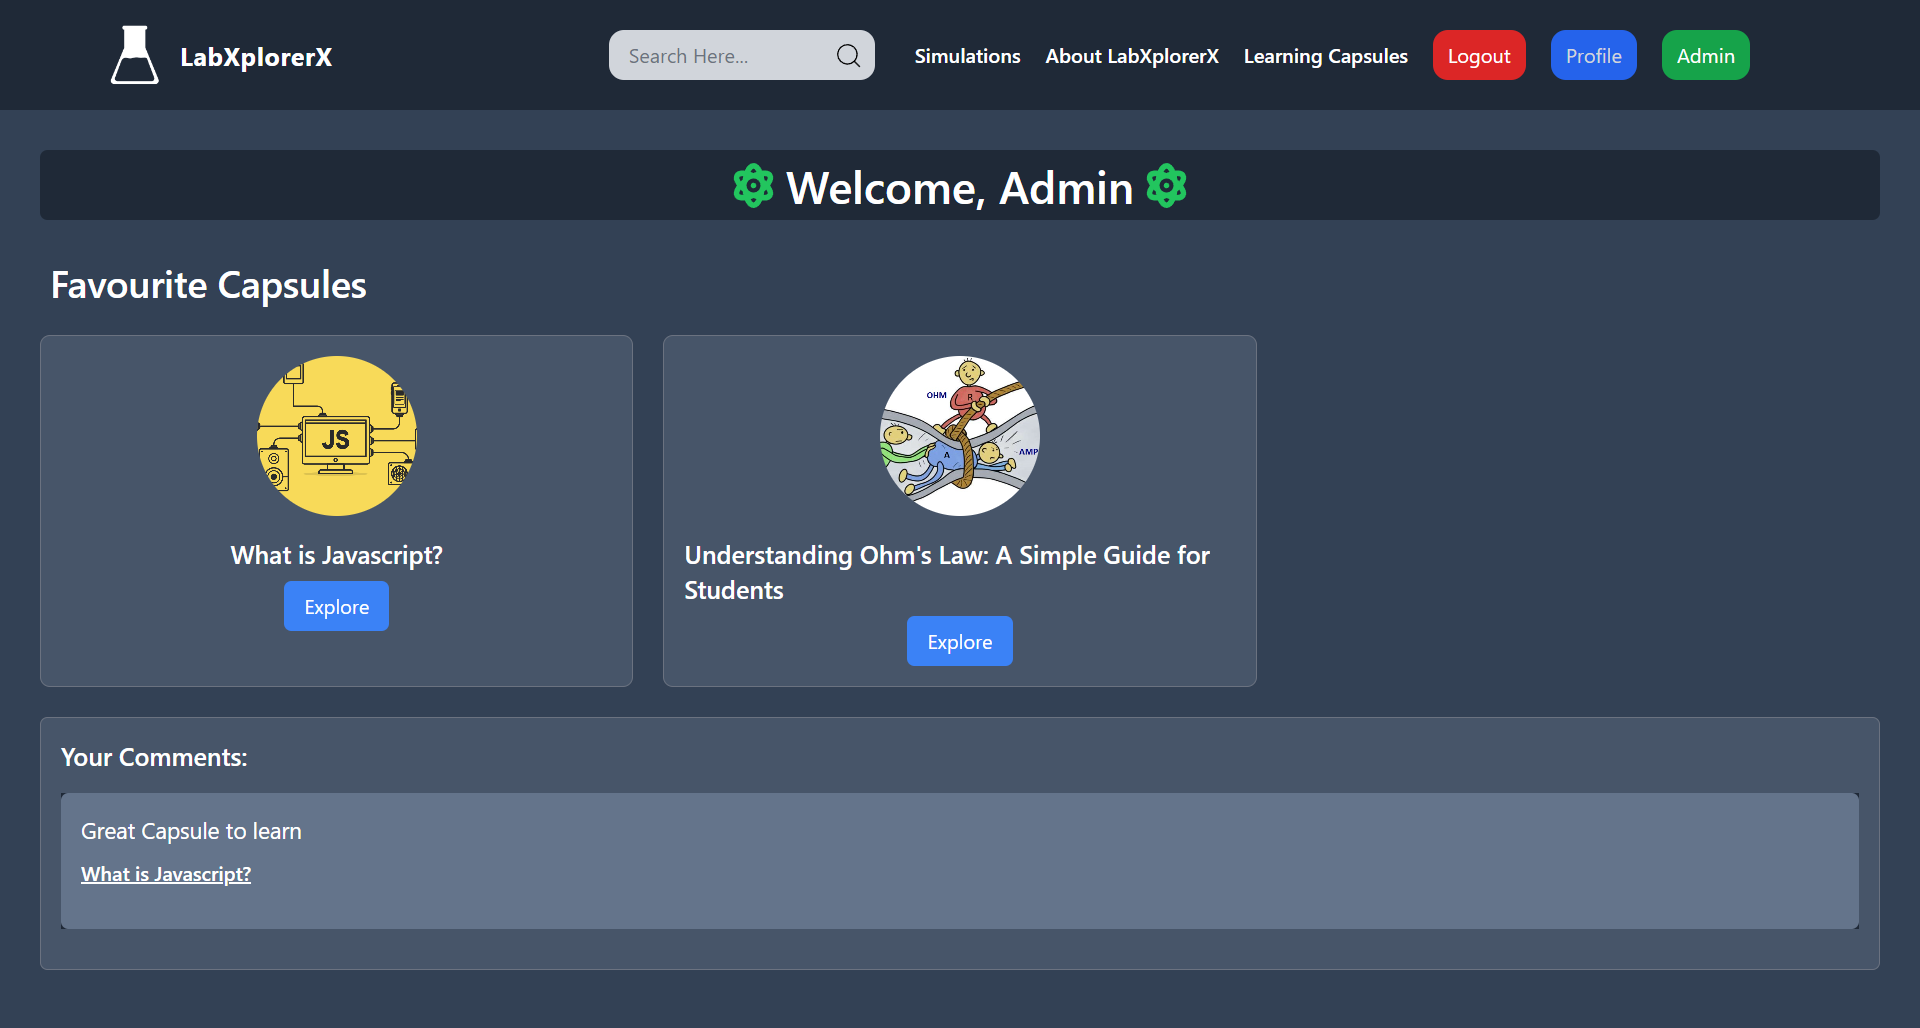
\includegraphics[width = 15cm]{Diagrams/output/profile.png}
    \caption{Profile}
\end{figure}

% Edit Quizzes Screen
\textbf{Edit Quizzes Screen:} Below is the screenshot of the Edit Quizzes Screen, used for creating, updating, and deleting quizzes.
\begin{figure}[H]
    \centering
    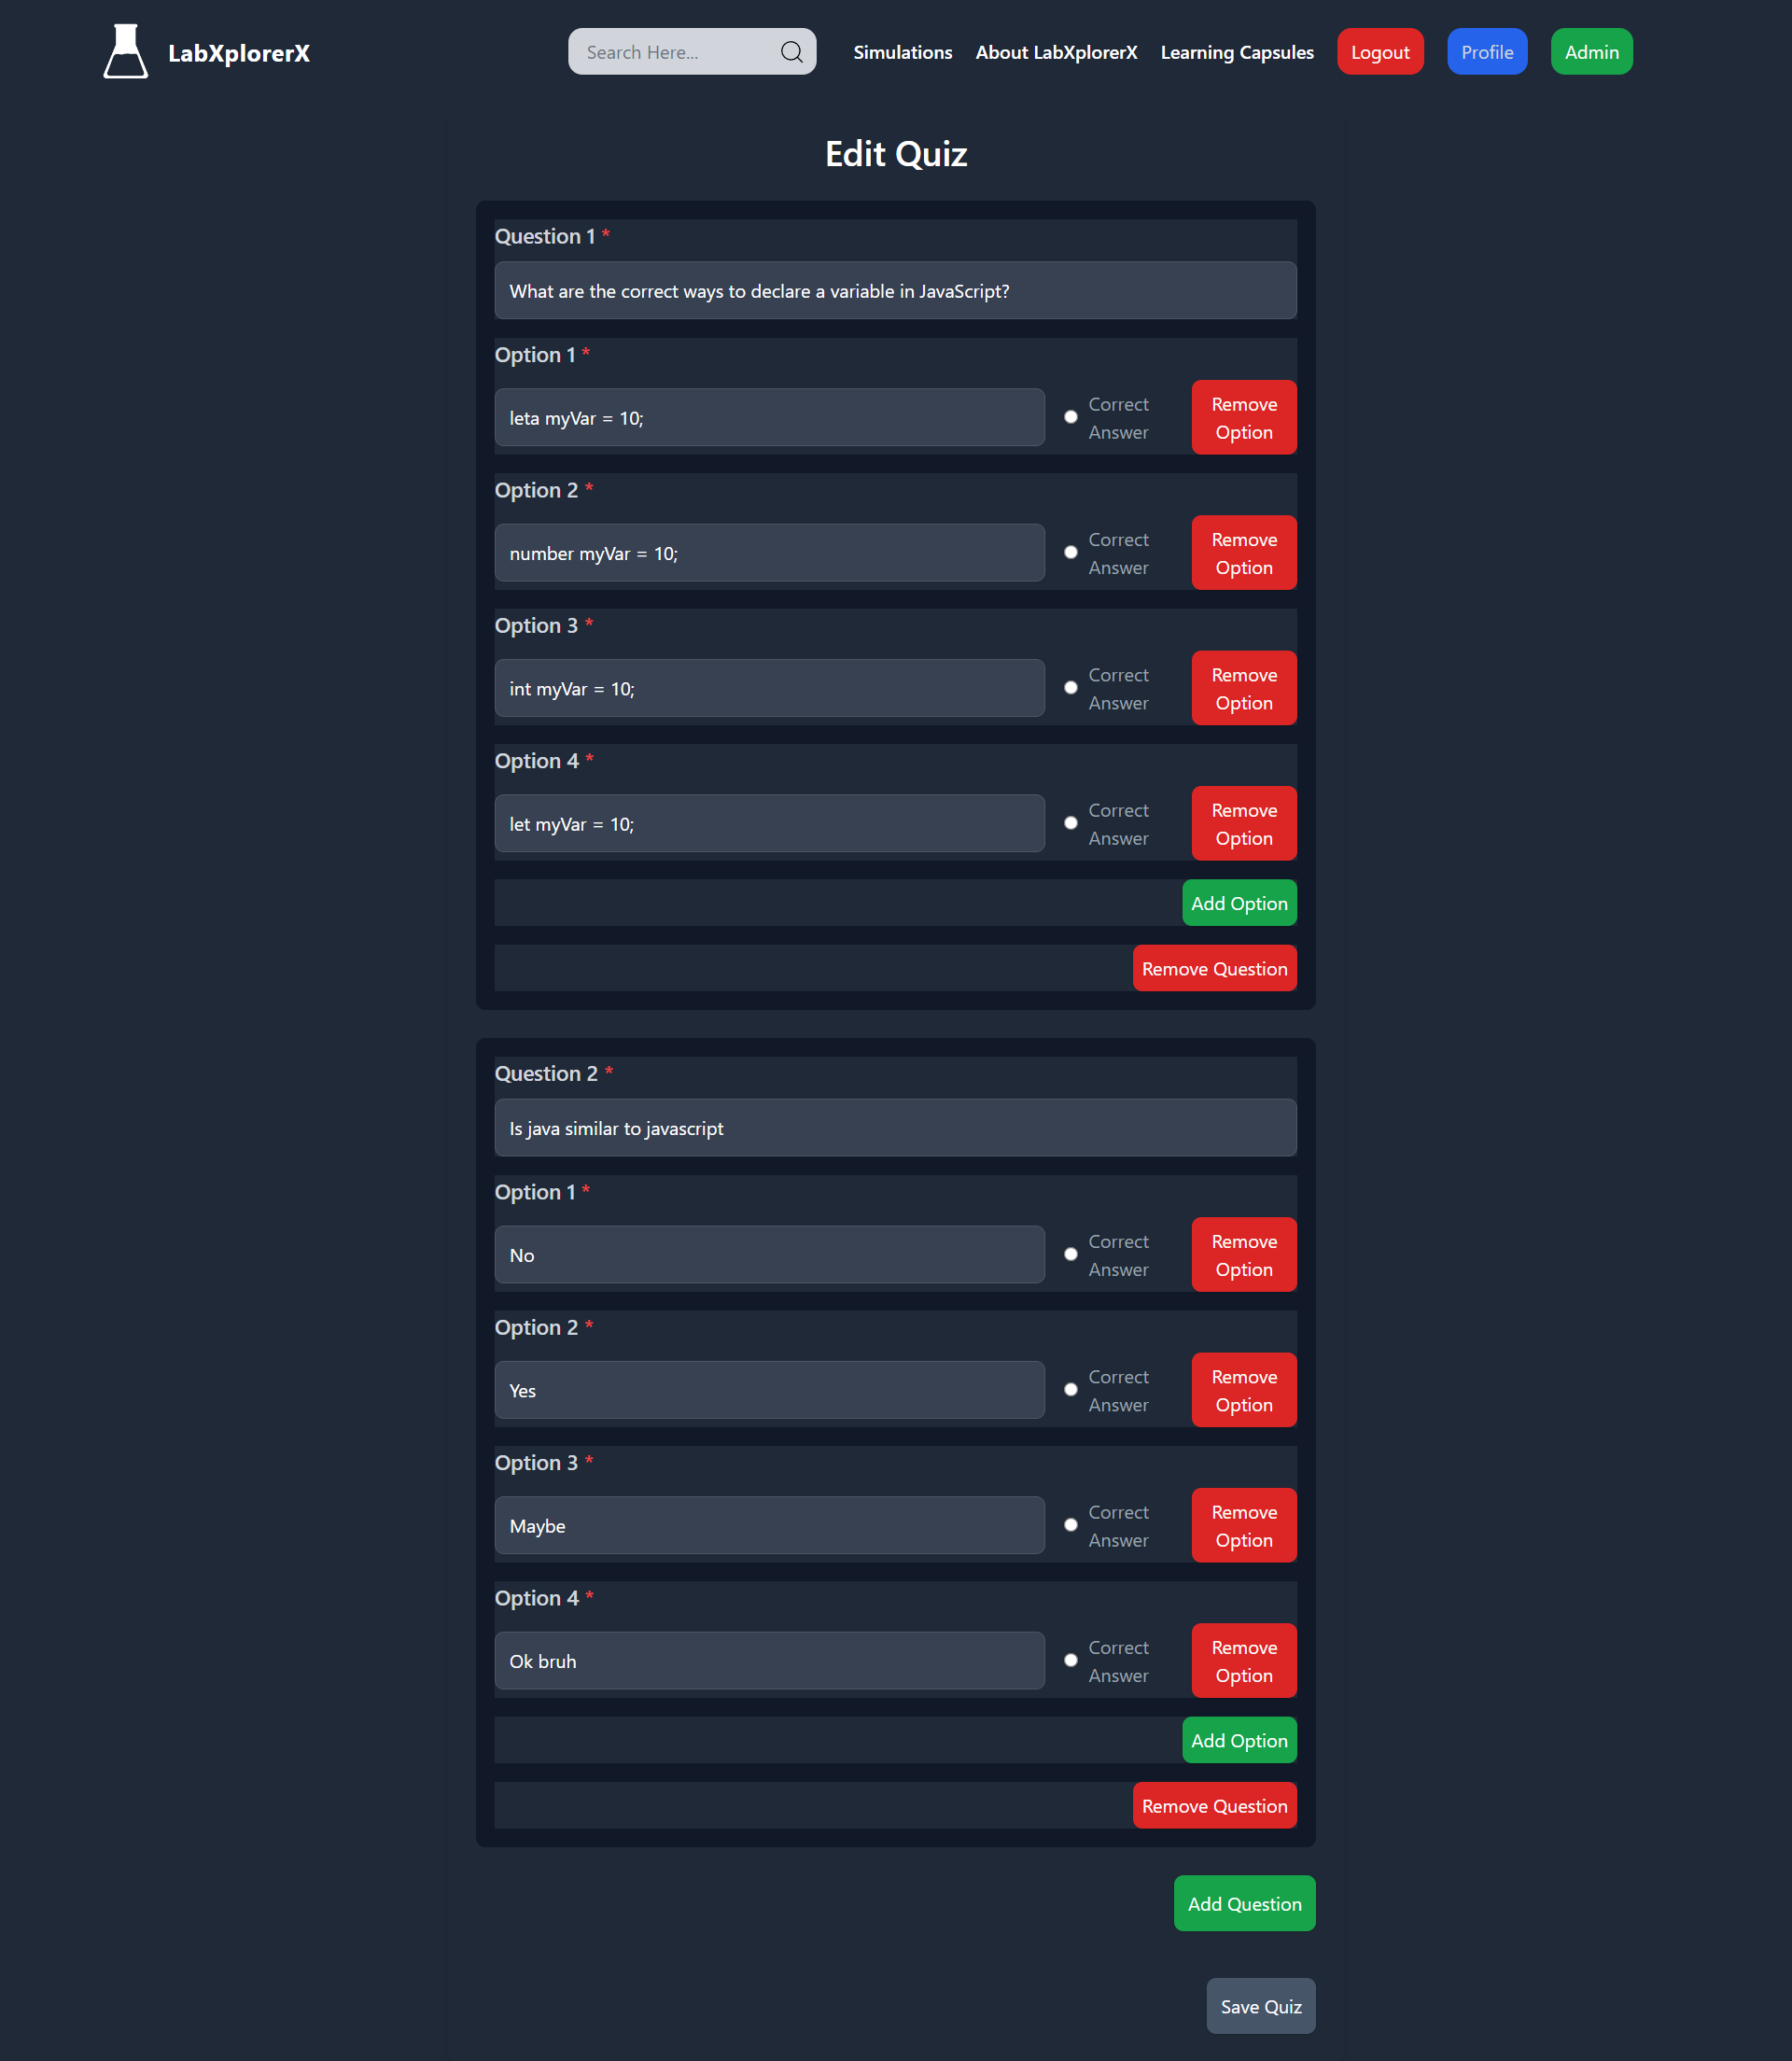
\includegraphics[width = 16cm]{Diagrams/output/edit_quiz.png}
    \caption{CRUD Quizzes}
\end{figure}
\newpage

% Search Results Screen
\textbf{Search Results Screen:} Below is the screenshot of the Search Results Screen, displaying results from user search queries.
\begin{figure}[H]
    \centering
    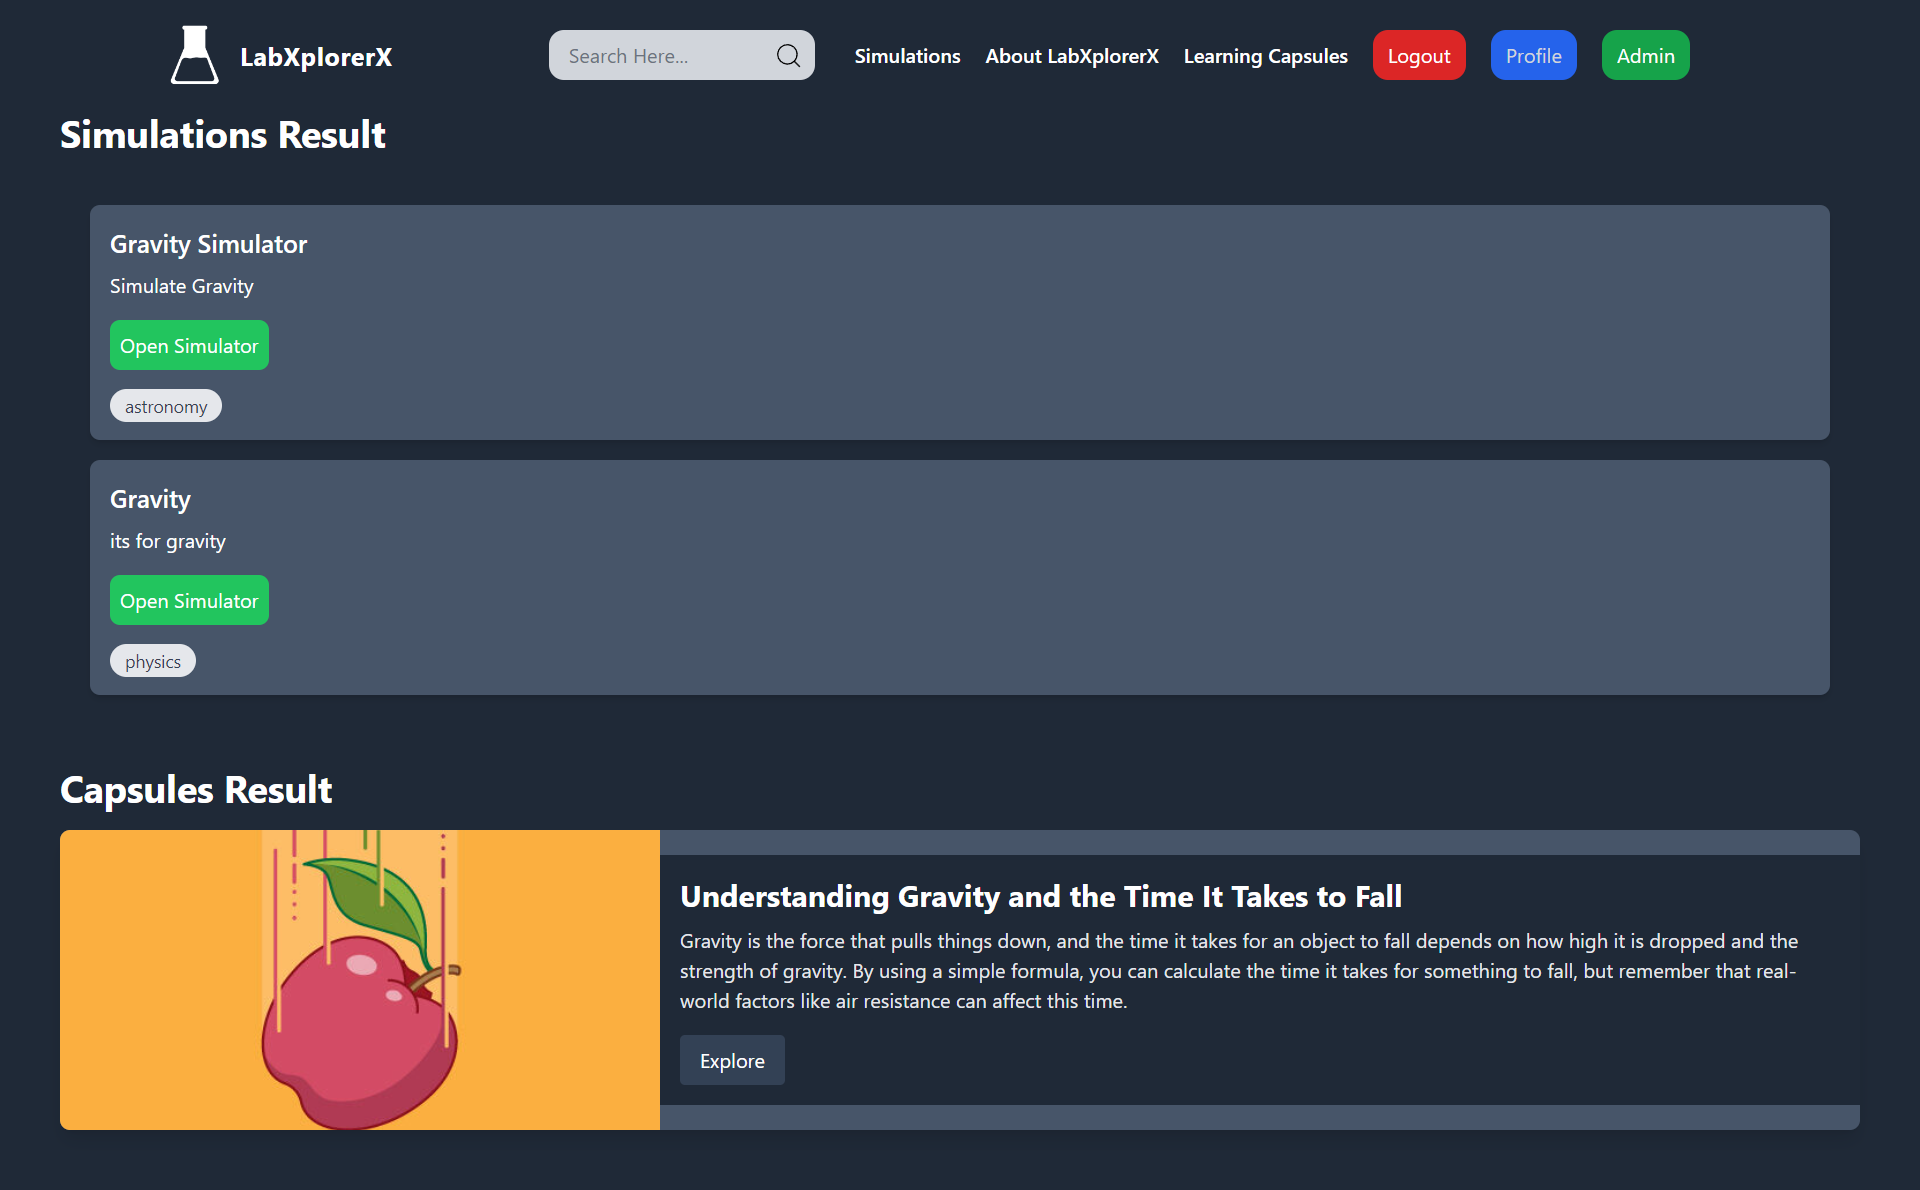
\includegraphics[width = 16cm]{Diagrams/output/search_results.png}
    \caption{Search Results}
\end{figure}
\textbf{Mail VerificationScreen:} Below is the screenshot of Main Verification link send to user while registering.
\begin{figure}[H]
    \centering
    
\includegraphics[width = 16cm]{Diagrams/output/verified.png}
    \caption{Search Results}
\end{figure}
\newpage
% Edit Capsule Screen
\textbf{Edit Capsule Screen:} Below is the screenshot of the Edit Capsule Screen, used for modifying details of existing capsules.
\begin{figure}[H]
    \centering
    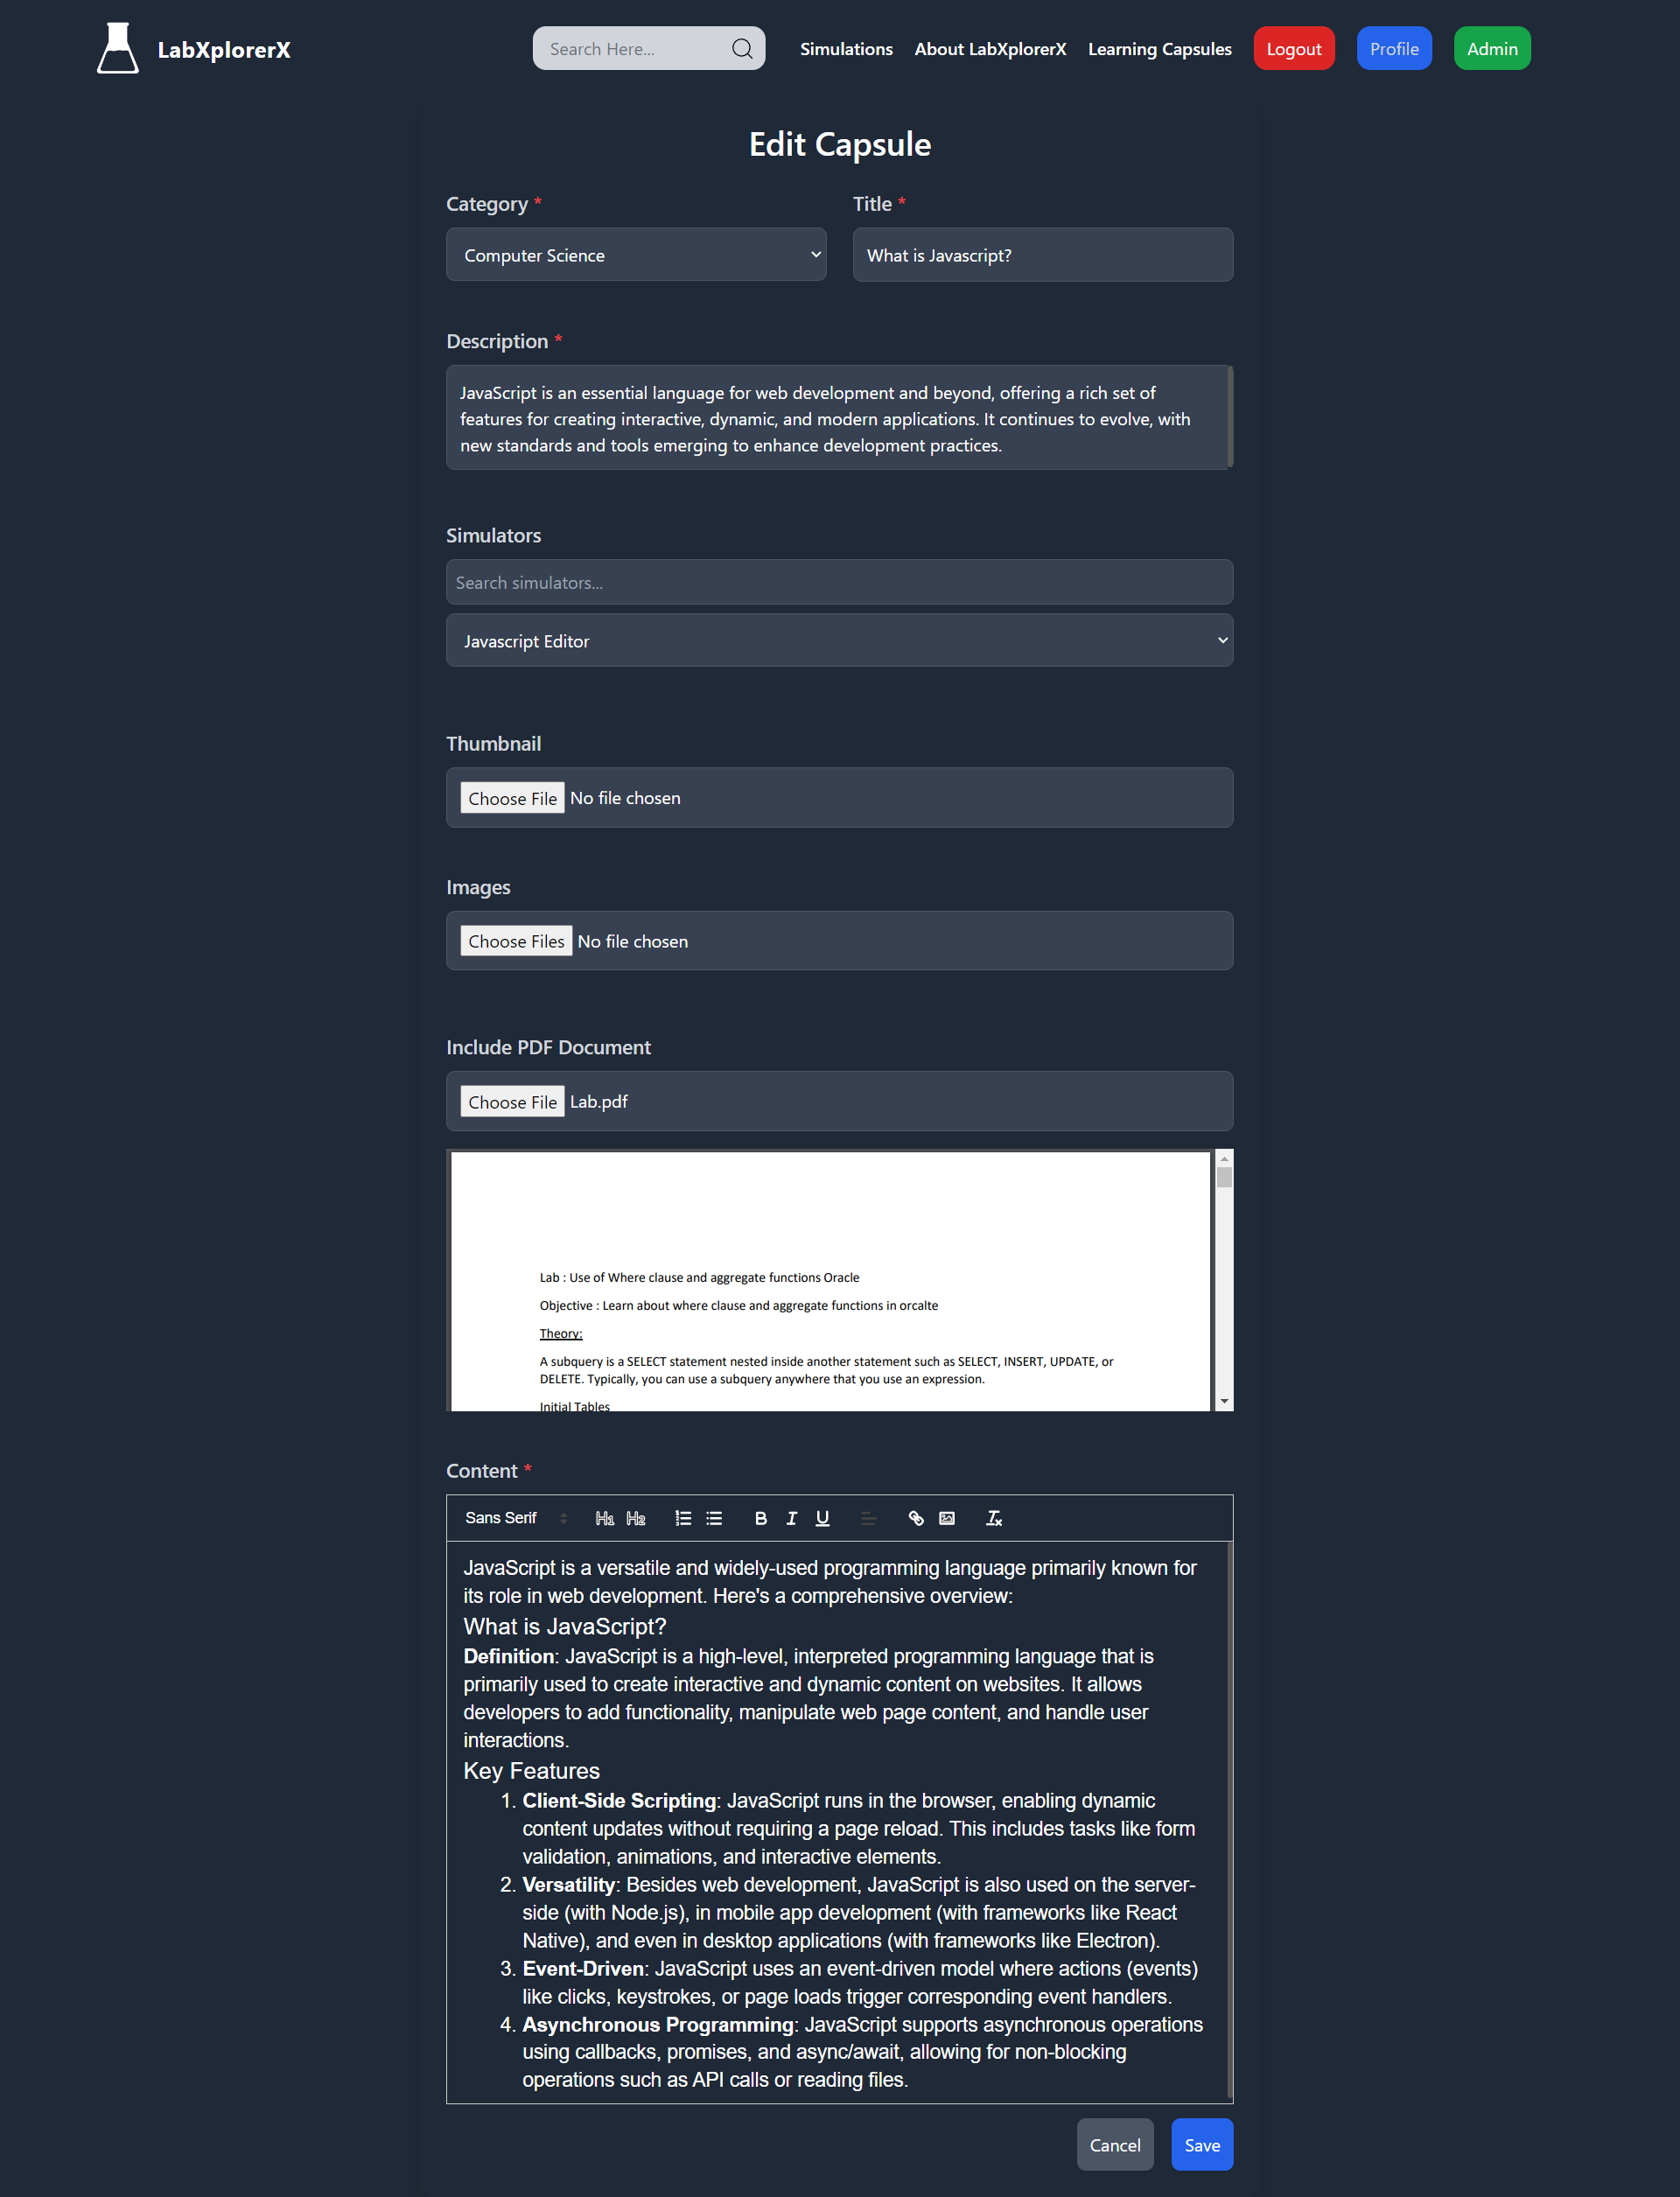
\includegraphics[width = 16cm]{Diagrams/output/edit_capsule.png}
    \caption{Edit Capsule}
\end{figure}

% Add Capsule Screen
\textbf{Add Capsule Screen:} Below is the screenshot of the Add Capsule Screen, where administrators can add new capsules.
\begin{figure}[H]
    \centering
    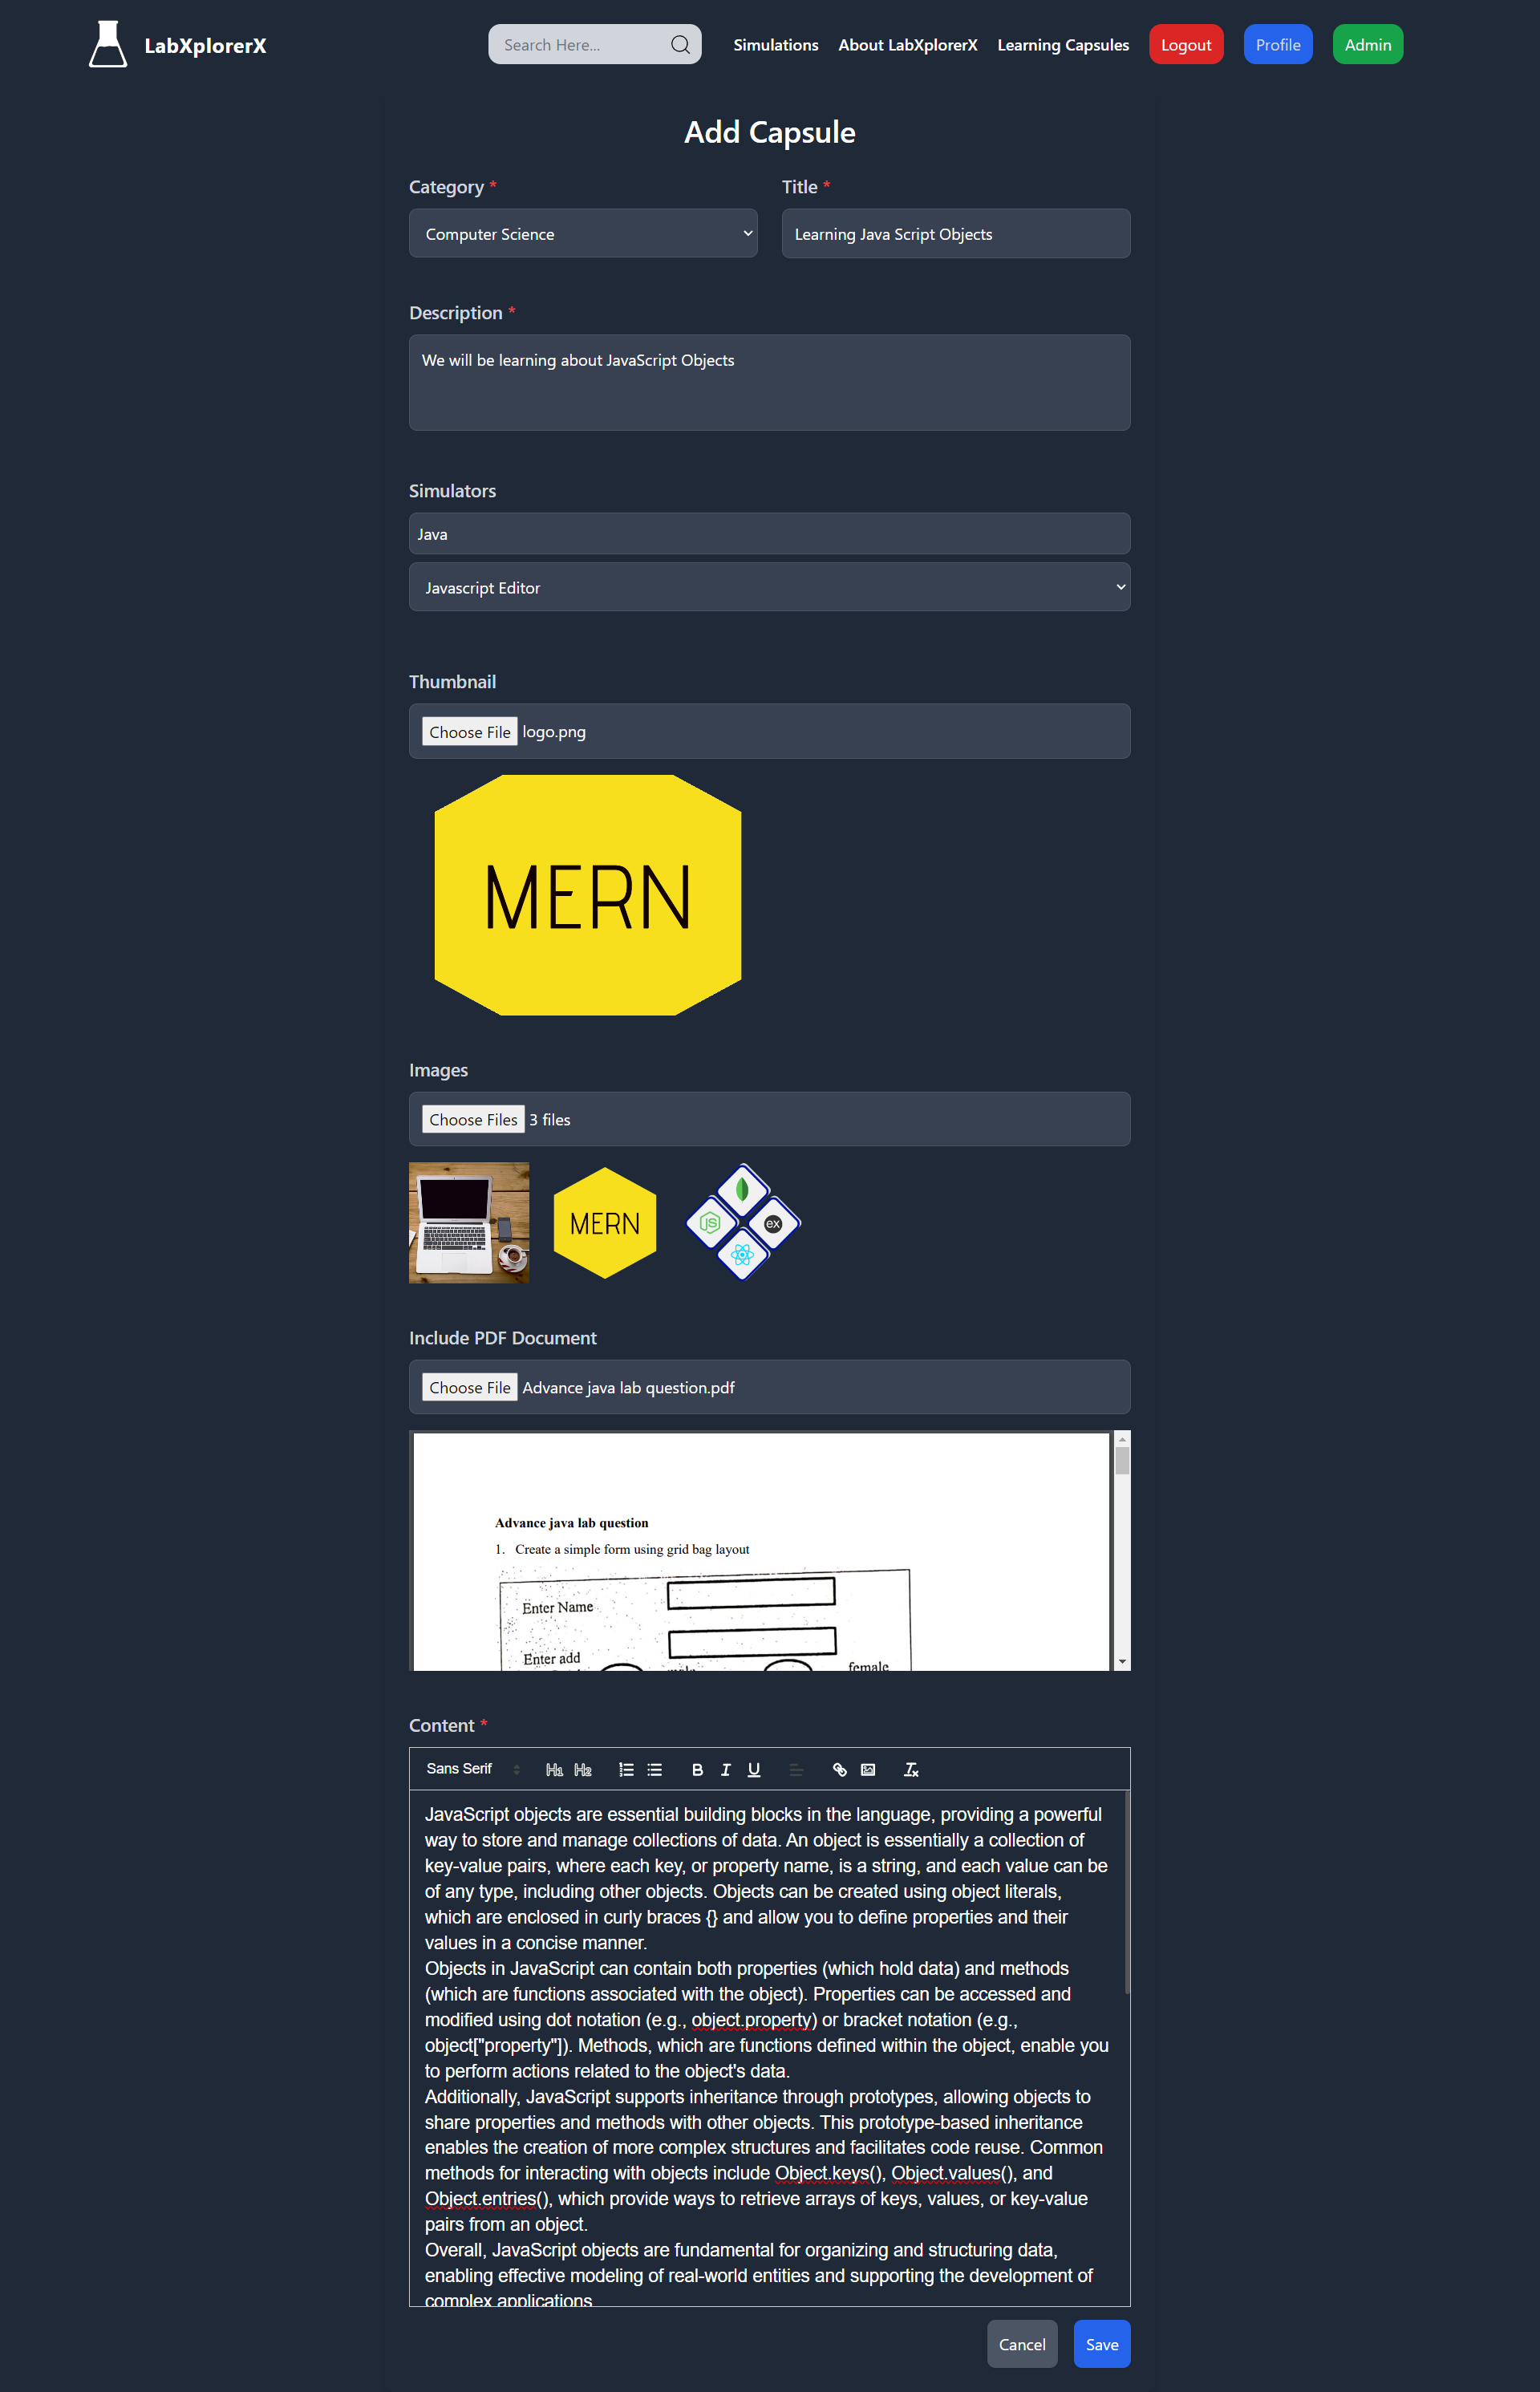
\includegraphics[width = 14cm]{Diagrams/output/addcapsule.png}
    \caption{Add Capsule}
\end{figure}

% After Addition of Capsule Screen
\textbf{After Addition of Capsule Screen:} Below is the screenshot of the screen displayed after a new capsule has been successfully added.
\begin{figure}[H]
    \centering
    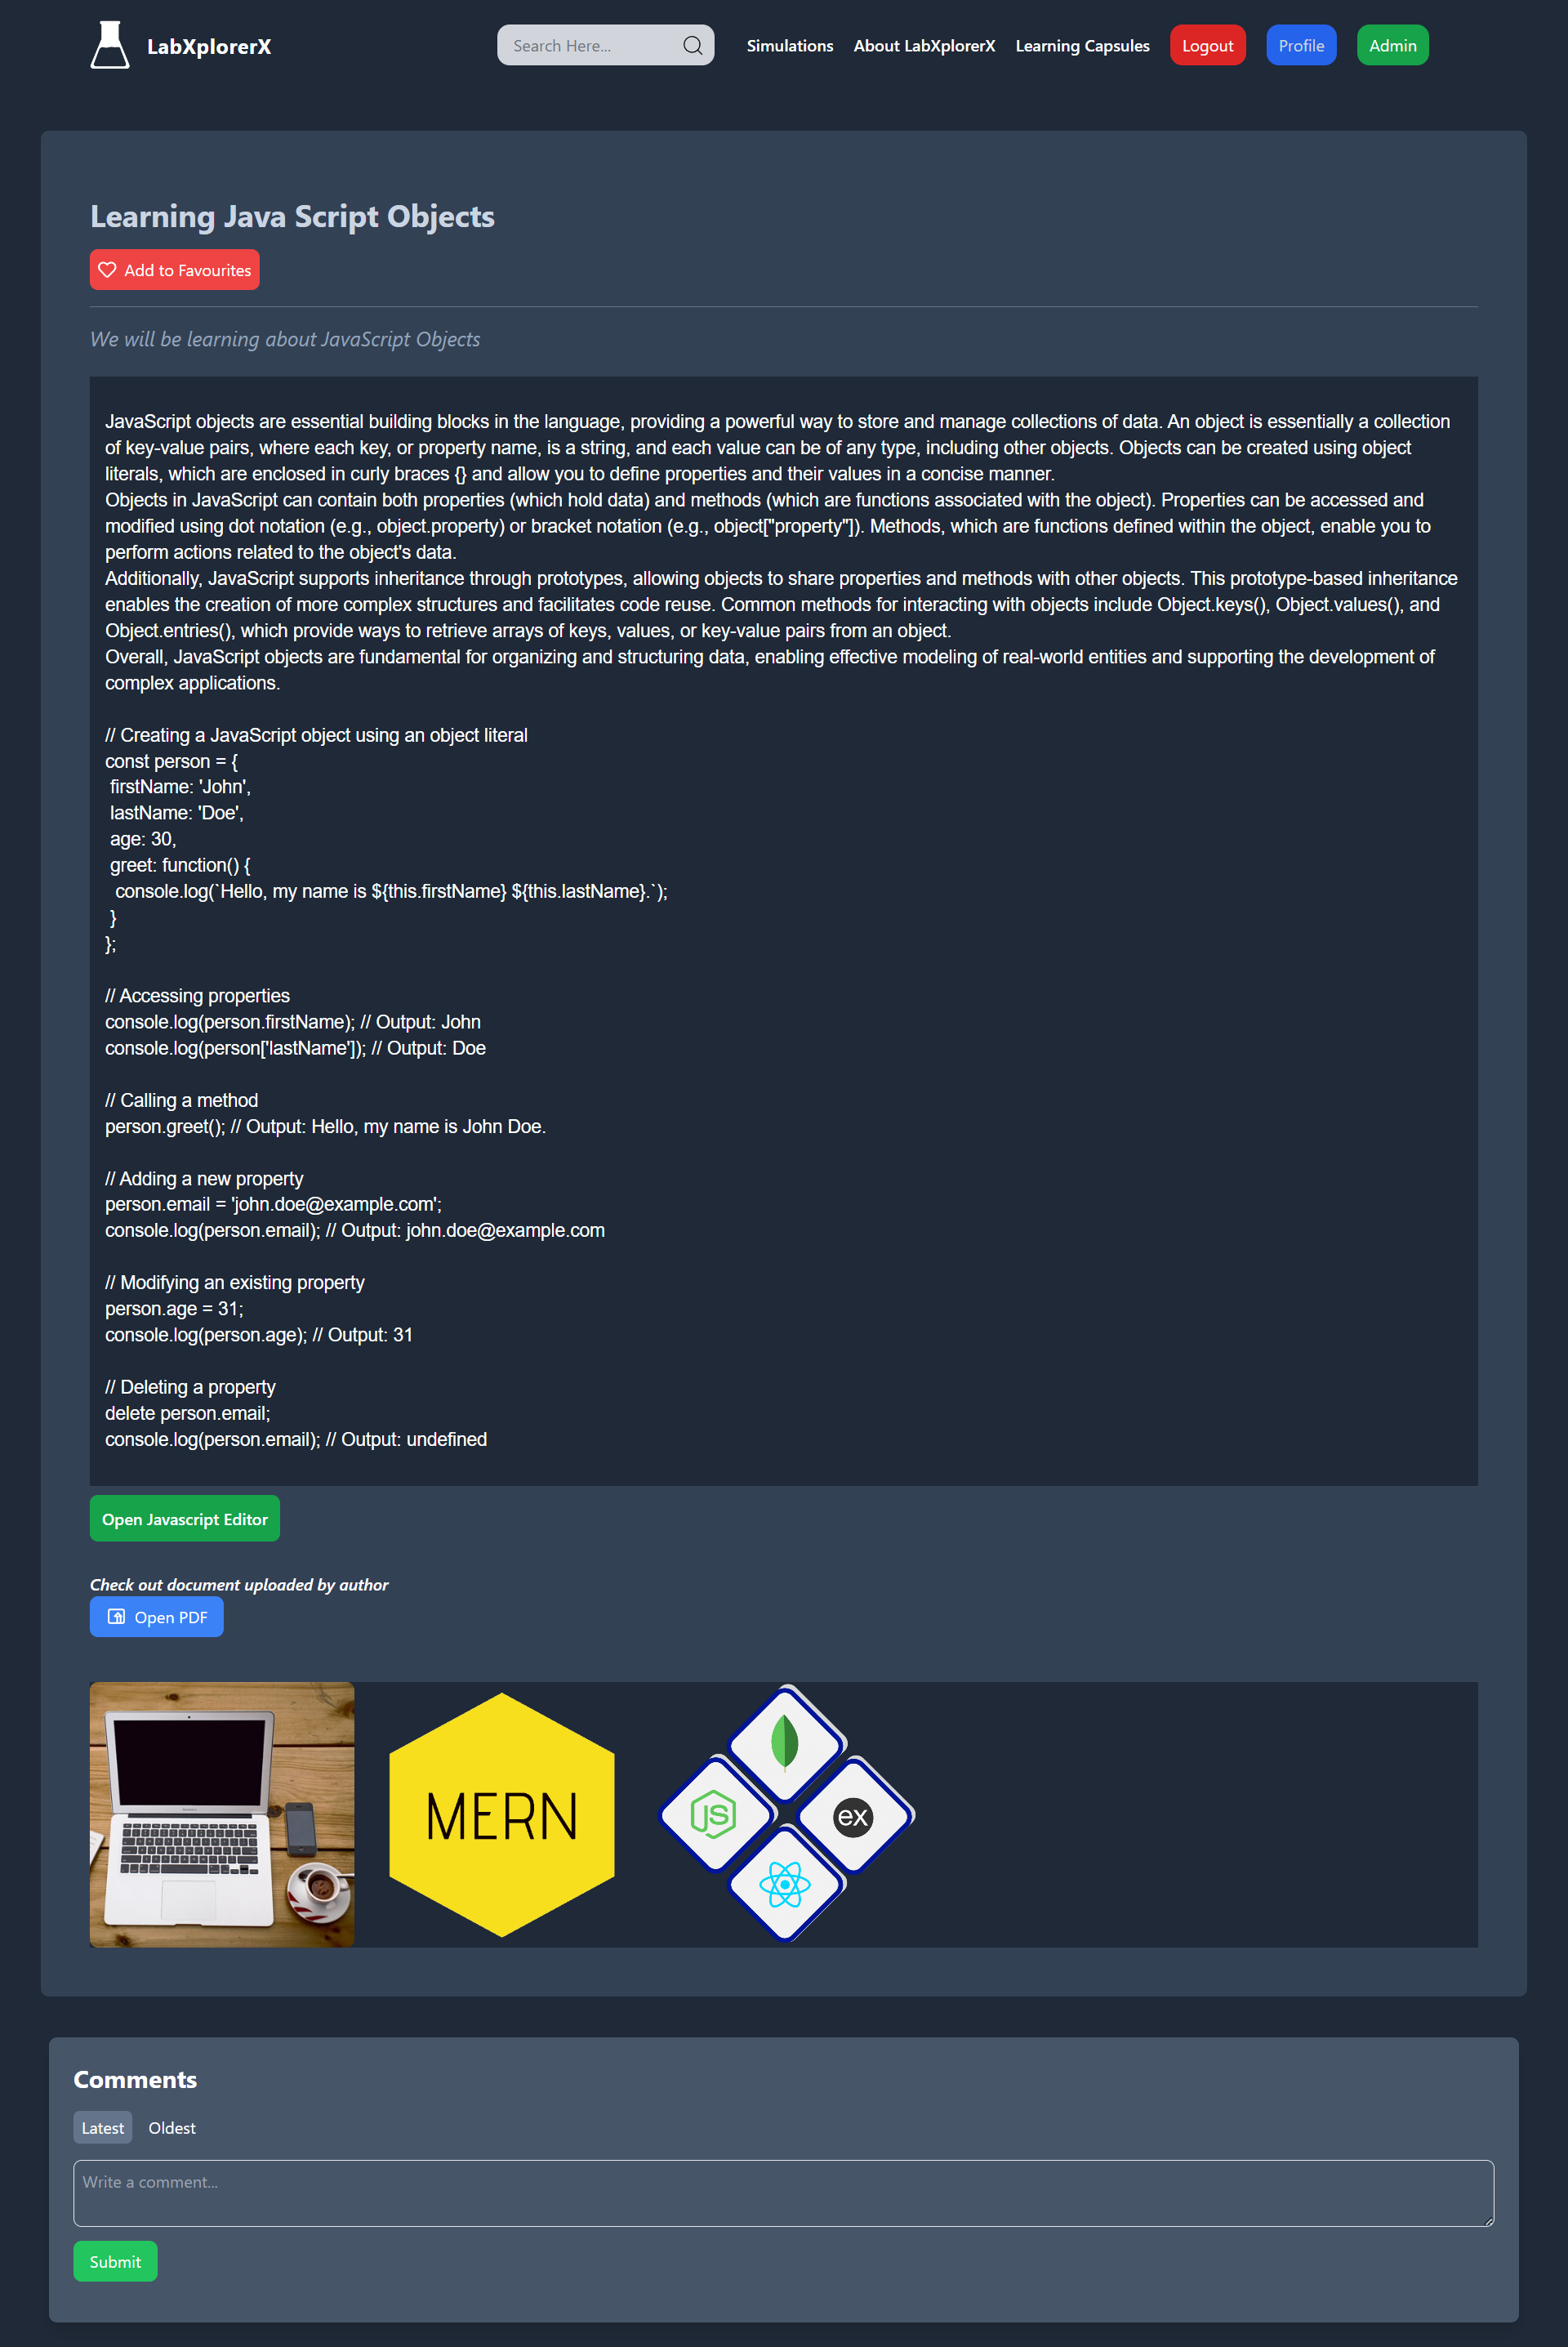
\includegraphics[width = 14cm]{Diagrams/output/after_addition.png}
    \caption{After Addition of Capsule}
\end{figure}

% Gravity Simulator
\textbf{Gravity Simulator:} Below is the screenshot of the Gravity Simulator, demonstrating the principles of gravity.
\begin{figure}[H]
    \centering
    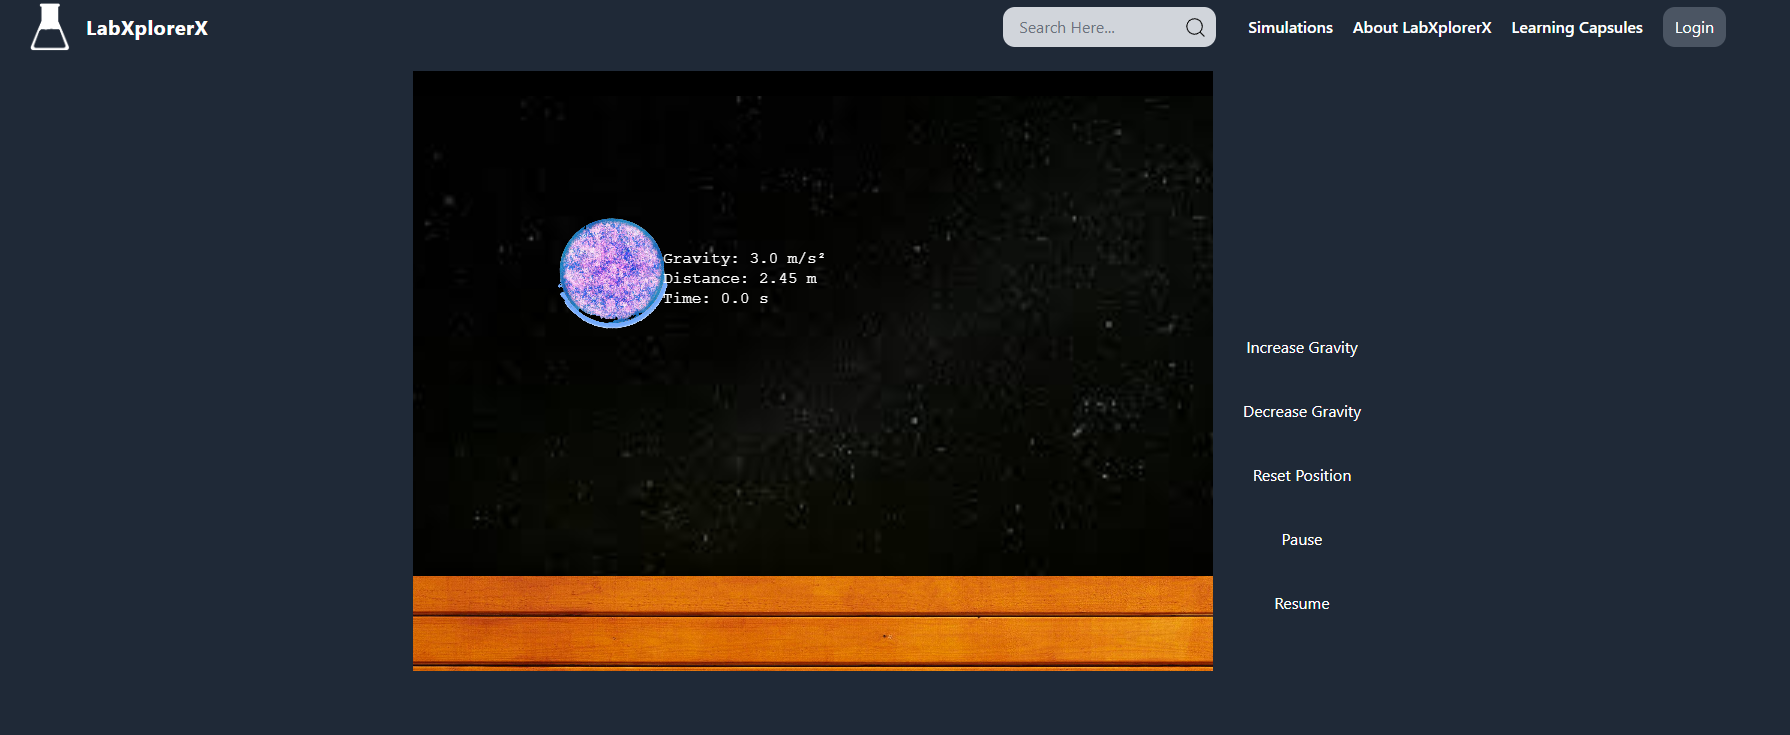
\includegraphics[width = 16cm]{Diagrams/output/gravity.png}
    \caption{Gravity Simulator}
\end{figure}

% Ohm's Law Simulator
\textbf{Ohm's Law Simulator:} Below is the screenshot of the Ohm's Law Simulator, illustrating Ohm's Law in an interactive format.
\begin{figure}[H]
    \centering
    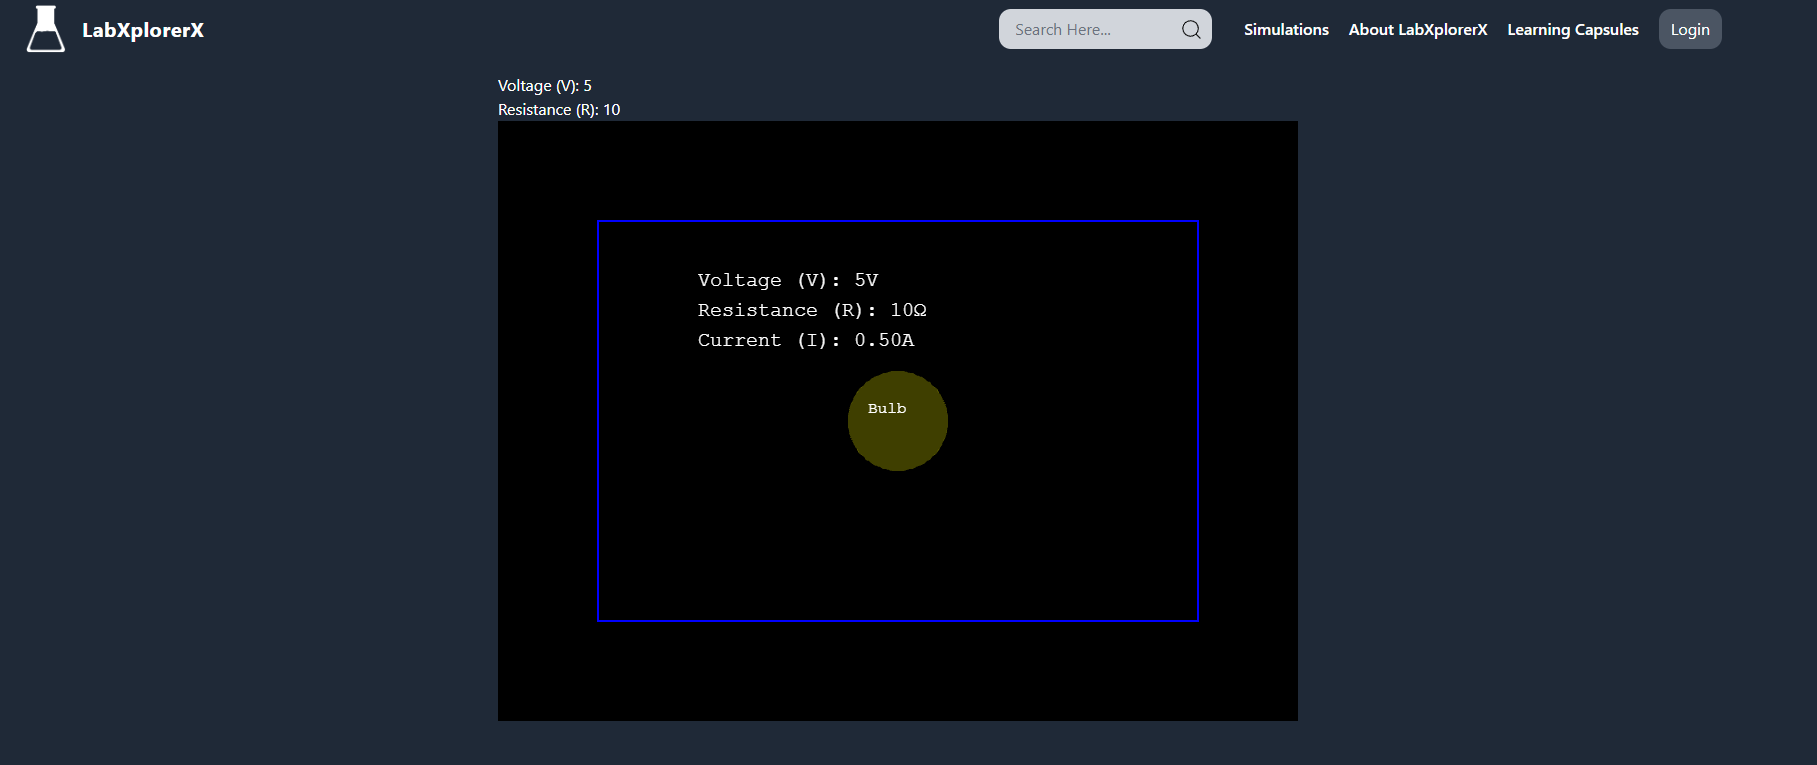
\includegraphics[width = 16cm]{Diagrams/output/ohms.png}
    \caption{Ohm's Law Simulator}
\end{figure}
\newpage

% Atom Simulator
\textbf{Atom Simulator:} Below is the screenshot of the Atom Simulator, allowing users to explore atomic structures.
\begin{figure}[H]
    \centering
    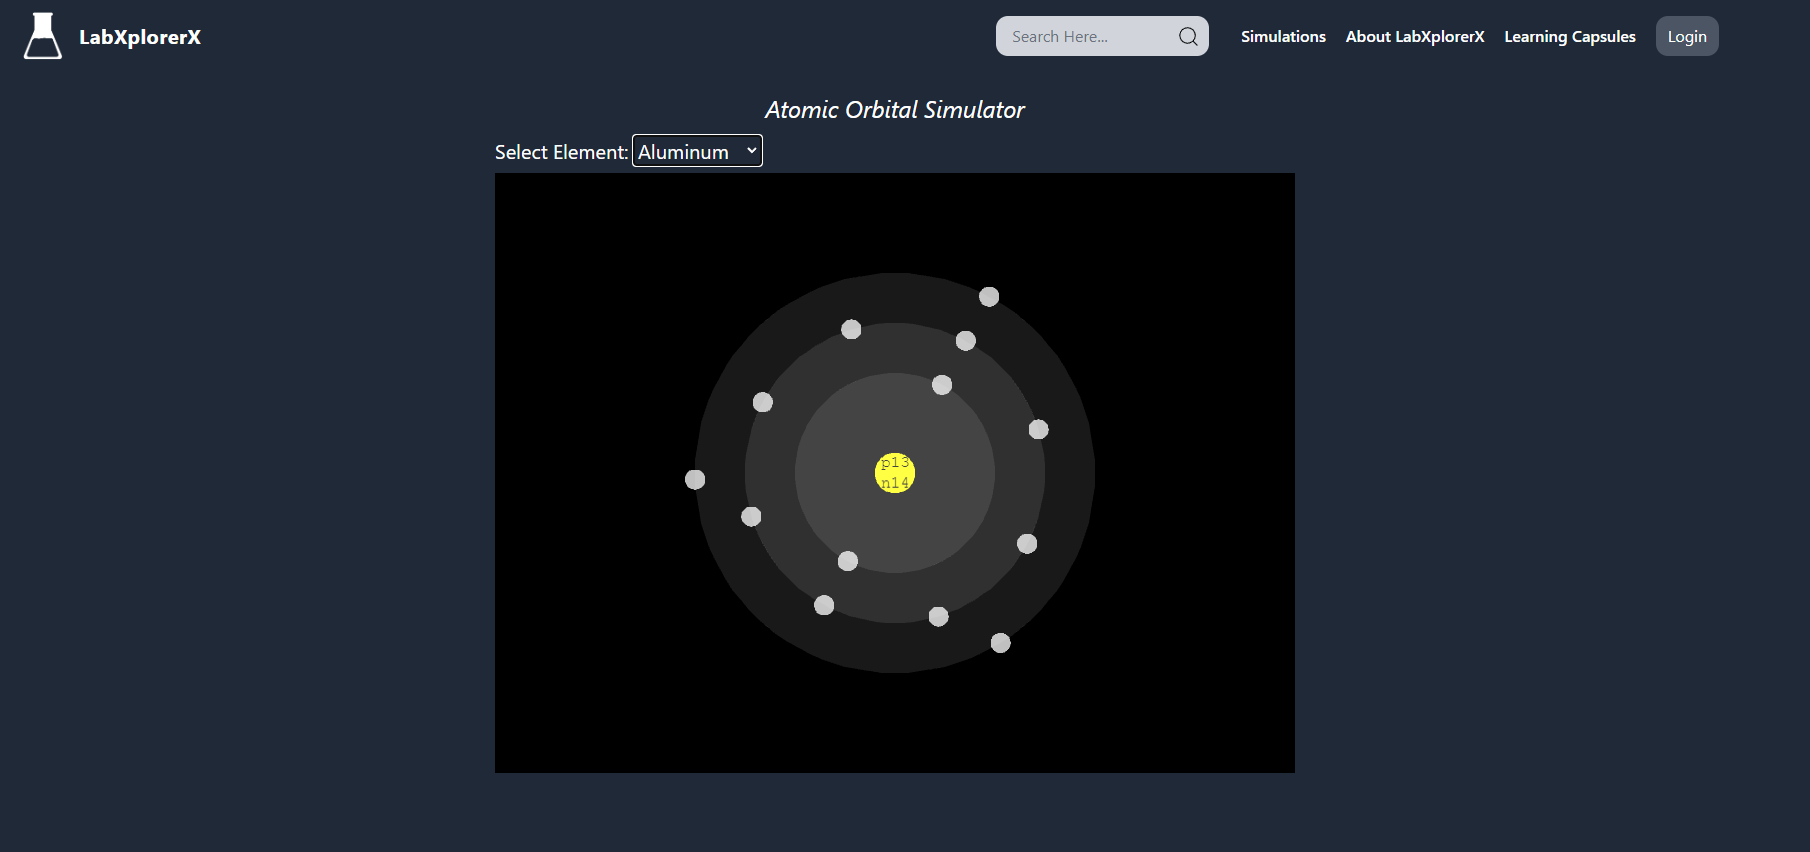
\includegraphics[width = 16cm]{Diagrams/output/atom.png}
    \caption{Atom Simulator}
\end{figure}

% Solar System Simulator
\textbf{Solar System Simulator:} Below is the screenshot of the Solar System Simulator, providing an interactive view of the solar system.
\begin{figure}[H]
    \centering
    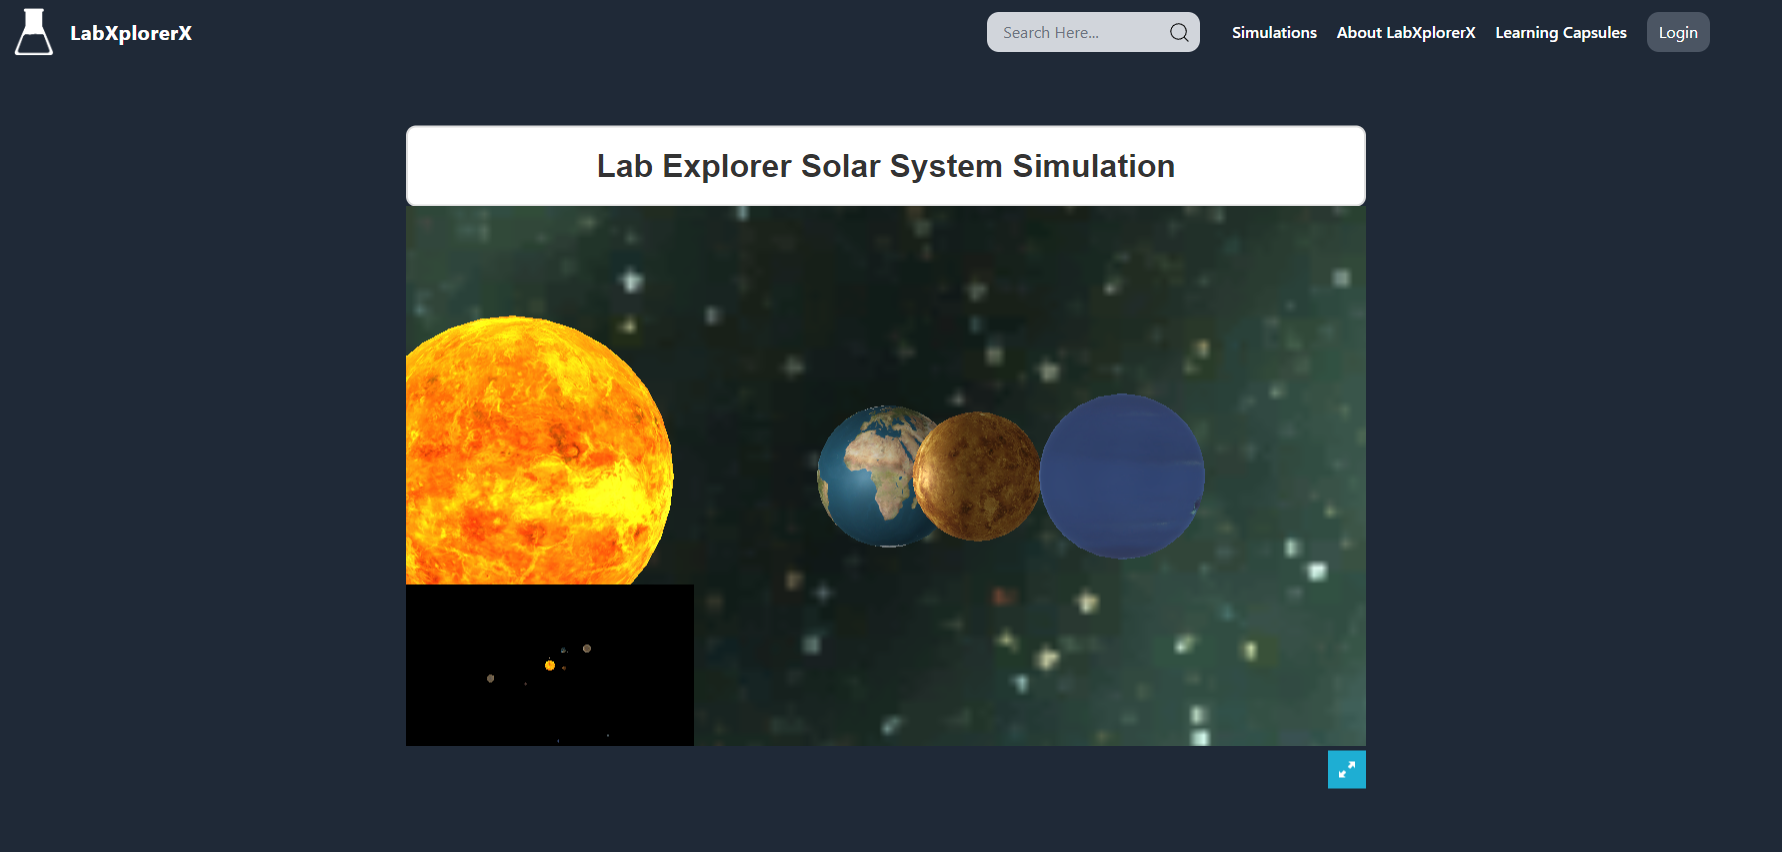
\includegraphics[width = 16cm]{Diagrams/output/solar.png}
    \caption{Solar System Simulator}
\end{figure}
\newpage

% JavaScript Editor
\textbf{JavaScript Editor:} Below is the screenshot of the JavaScript Editor, where users can write and test JavaScript code.
\begin{figure}[H]
    \centering
    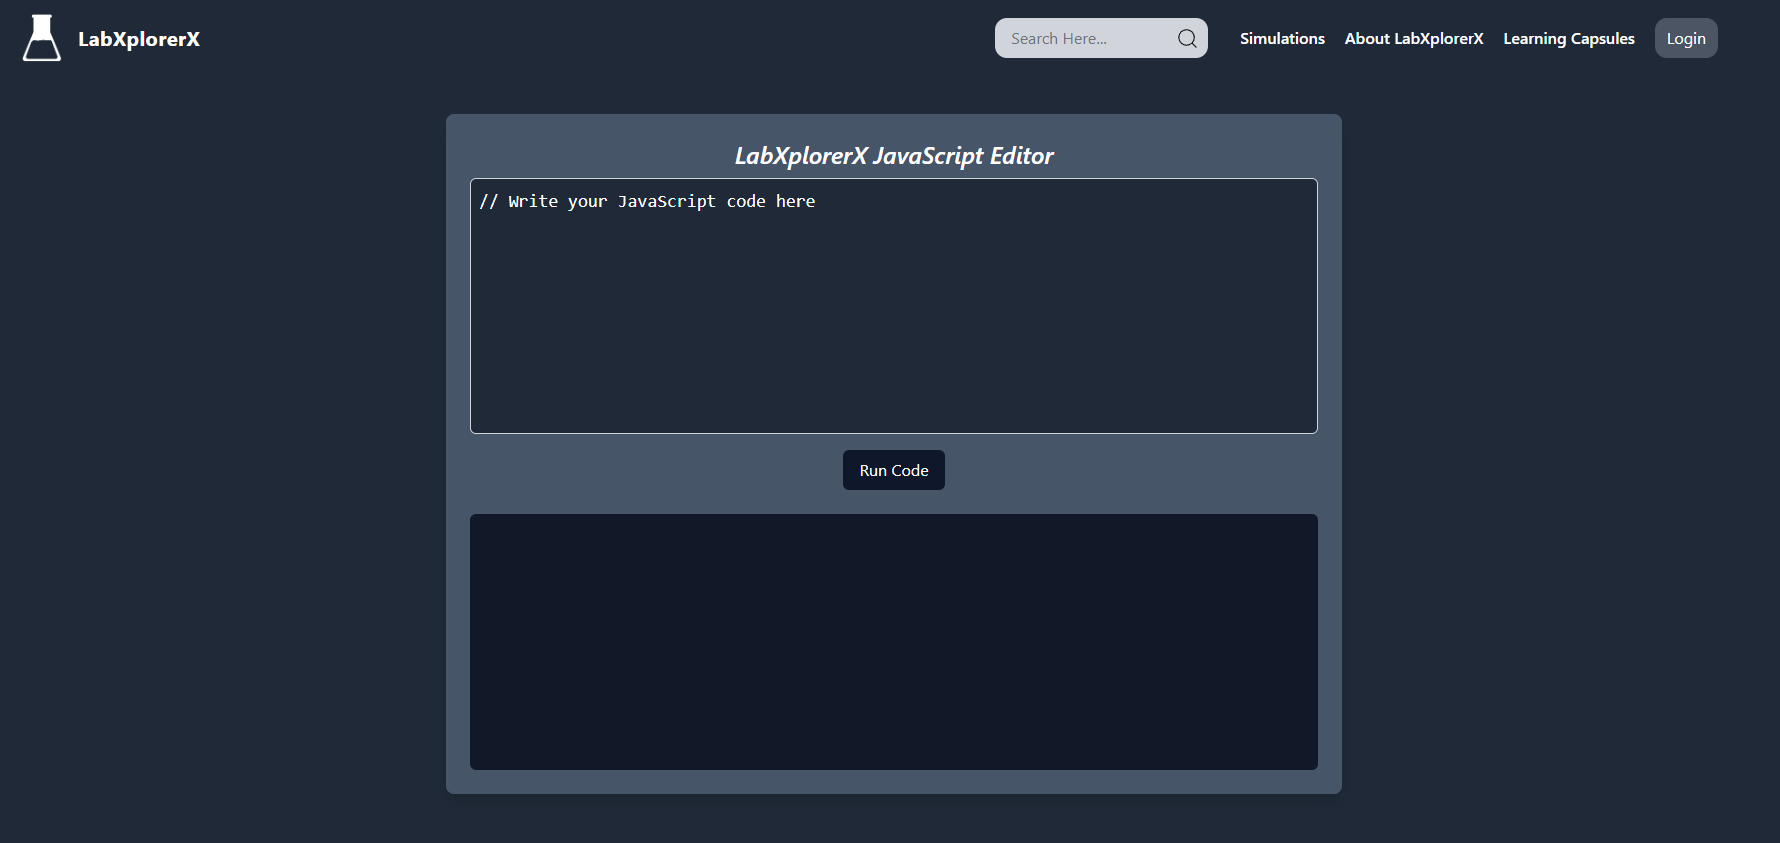
\includegraphics[width = 16cm]{Diagrams/output/js.png}
    \caption{JavaScript Editor}
\end{figure}


\section{Future Recommendations}

While the implementation of LabXplorerX is complete, several enhancements could further improve the platform:

\begin{itemize}[leftmargin=1cm]
    \item \textbf{Additional Simulations:} Expand the range of simulations by developing new ones. This will provide a broader scope of interactive learning experiences and cover more subjects.
    
    \item \textbf{Responsive Design for Simulations:} Enhance the responsiveness of existing simulations to ensure optimal performance across different devices and screen sizes. This improvement will make the simulations more accessible and user-friendly on mobile and tablet devices.
    
    \item \textbf{Extended Profile Functions:} Introduce additional features to user profiles, such as advanced progress tracking, customizable learning paths, and enhanced account management options. This will further personalize and improve the learning experience for students.
\end{itemize}